\chapter{ANÁLISIS DE RESULTADOS}

En este capítulo se presenta el análisis y discusión de los principales resultados 
obtenidos en el desarrollo de este proyecto. Del análisis por elementos finitos 
se presentan los resultados del caso bidimensional y del modelo tridimensional, comparando 
ambos casos, con la finalidad de discutir la viabilidad de utilizar un análisis de tipo 
deformación plana en una simulación de formado como esta. Además, los resultados del 
análisis numérico se comparan con lo obtenido mediante el análisis experimental.\\

% Además, con la finalidad de determinar algunas condiciones o parámetros que faciliten 
% el análisis de procesos de formado de este tipo, se presenta una sección destinada 
% a evaluar la influencia del escalamiento de masa selectivo cuya utilidad va en 
% dirección de disminuir el tiempo de cómputo requerido. Asimismo se expone una sección 
% referente al uso de algunos modelos de material como el bilineal isotrópico y cinemático, 
% la plasticidad cinemática y curvas multilineales, para determinar si las variaciones 
% en el comportamiento del material son significativas.

\section{Análisis por el método de elementos finitos}

\subsection{Análisis 2D}

% \subsubsection{Estatus global}

Normalmente en un análisis de tipo dinámico explícito, el balance de energía juega 
un papel importante e incluso puede utilizarse como criterio de \textit{terminación}. 
Para considerar que un análisis es aceptable, la energía cinética debe representar 
menos de un 5 \% de la energía interna del modelo, de lo contrario, los efectos 
inerciales inducidos podrían afectar de manera considerable tanto la geometría 
resultante como los datos de salida. En la figura \ref{fig:energy_status_01} se observa 
que la energía cinética representa un porcentaje menor al 1\% de la energía interna, lo 
cual implica que el análisis está dentro del rango aceptable. \\

\begin{center}
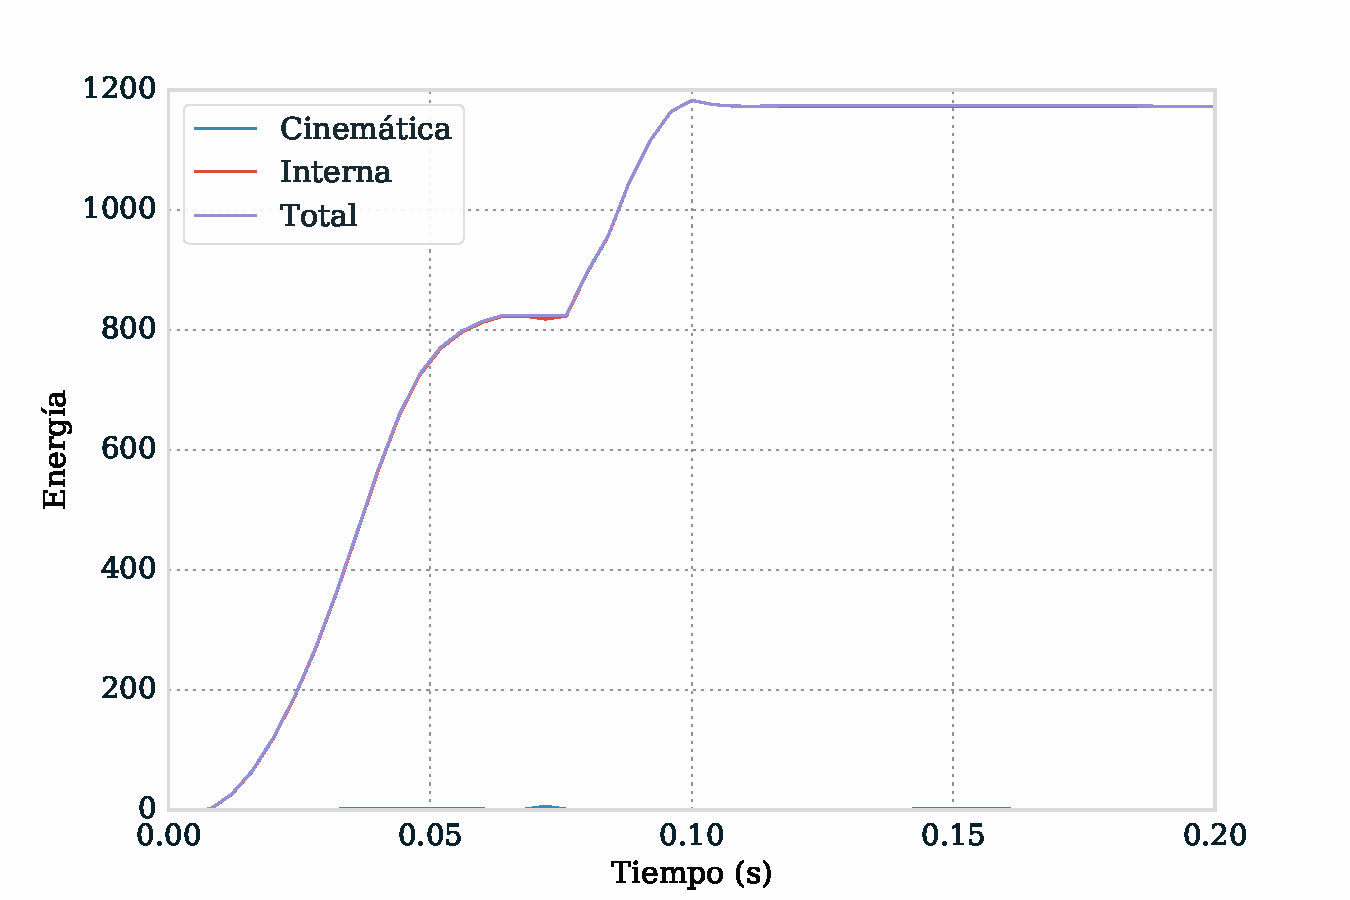
\includegraphics[width=0.8\textwidth]{src/ch4/energy_status_01.pdf}
\captionof{figure}{Variación de la energía total, interna y cinemática, primer paso}
\label{fig:energy_status_01}
\end{center}

El elemento \texttt{PLANE162}, utilizado en el mallado para el análisis bidimensional, 
tiene sólo un punto de integración, lo cual le hace robusto para grandes deformaciones 
y permite un ahorro significativo de tiempo computacional, pero esto mismo les hace 
propensos a presentar modos de energía cero. Estos modos, comúnmente referidos como 
modos de Hourglass, son de naturaleza oscilatoria y tienen periodos mucho más pequeños 
que la respuesta estructural de un sistema, resultando en estados matemáticos que físicamente 
no son posibles y que normalmente tienden a deformar la malla en forma de zigzag.
Para verificar que la deformación de Hourglass no ha influido de manera considerable 
en un análisis se debe comparar la energía interna del modelo con la energía de Hourglass, 
esta última no debe ser mayor al 10\% de la primera para considerar aceptable los 
resultados de la simulación ~\cite{lsdyna-ansys-manual}. En la gráfica de la figura \ref{fig:hourglass_internal_01} 
se muestra la energía interna vs la energía de Hourglass y se aprecia que la proporción 
varía en un rango del 1.5 a 2\%, lo cual indica que la deformación de Hourglass se encuentra 
dentro de los límites aceptables.

\begin{center}
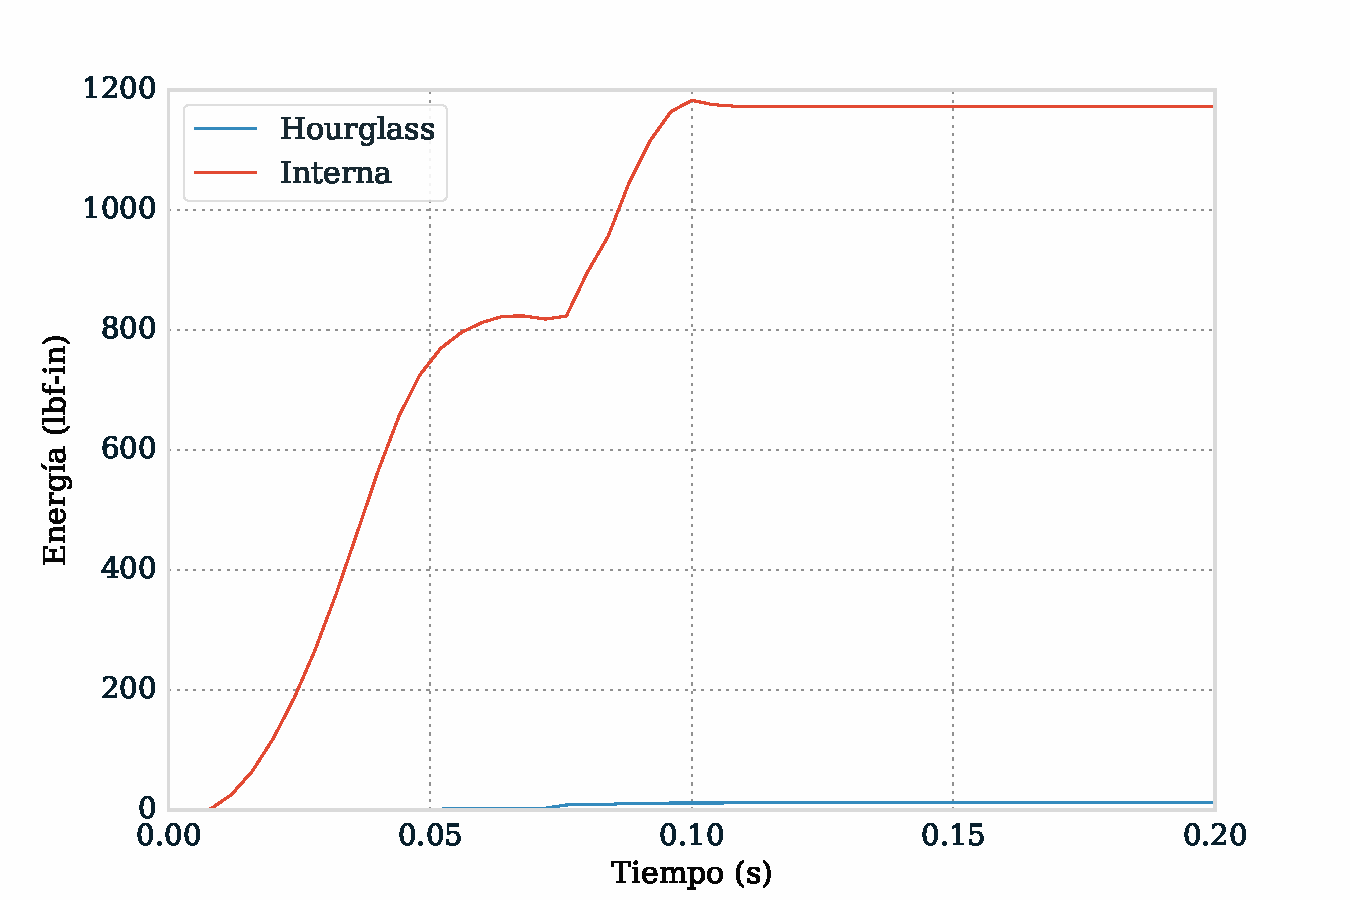
\includegraphics[width=0.8\textwidth]{src/ch4/hourglass_internal_01.pdf}
\captionof{figure}{Comparación energía interna vs energía de Hourglass}
\label{fig:hourglass_internal_01}
\end{center}


\subsubsection{Geometría resultante}

% En la figura \ref{fig:shape_sequence_01} se muestra la secuencia de formado 
% de la geometría resultante, se puede apreciar el doblado en U y el doblado 
% llevado a cabo por las levas.

% \begin{center}
% 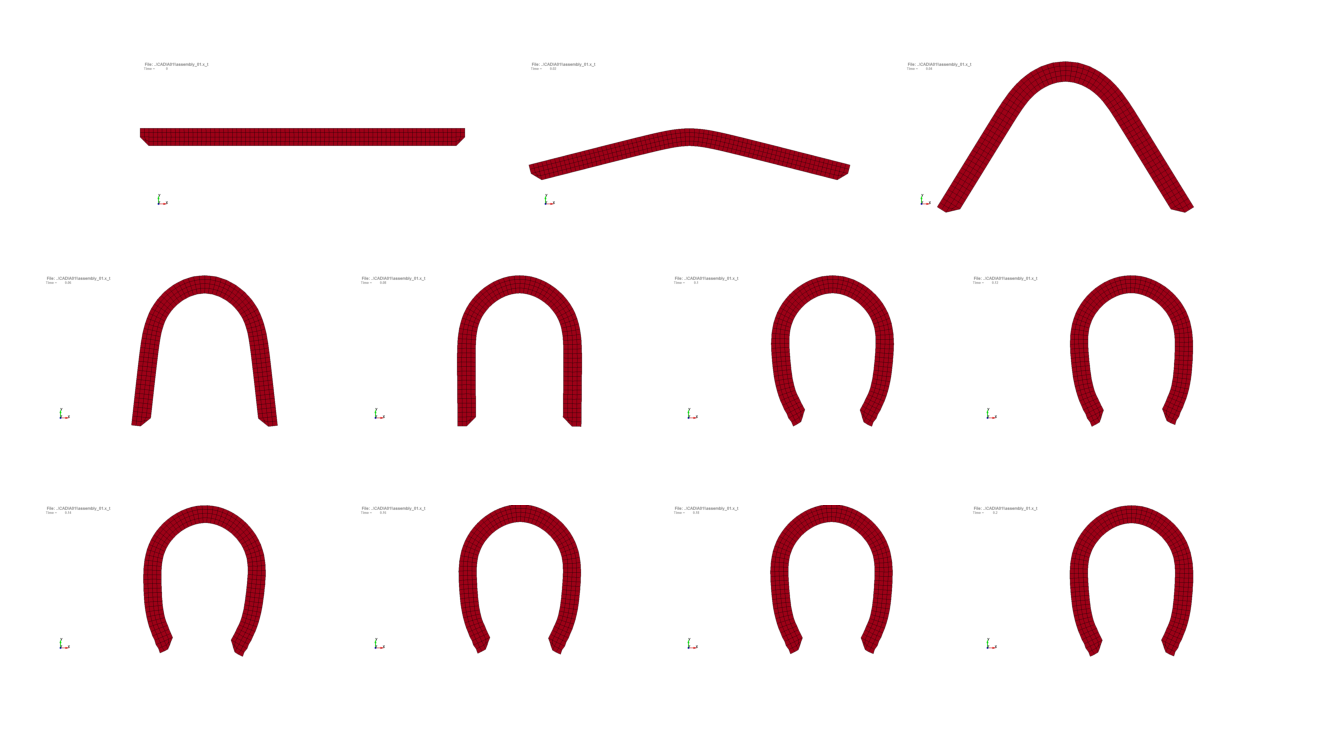
\includegraphics[width=0.95\textwidth]{src/ch4/shape_sequence_01.pdf}
% \captionof{figure}{Secuencia de la geometría resultante}
% \label{fig:shape_sequence_01}
% \end{center}

Las figuras \ref{fig:geometry_01} y \ref{fig:geometry_02} muestran las geometrías 
resultantes al final del primer y segundo paso del proceso de formado. Las formas 
obtenidas corresponden a lo esperado cuando se diseñó el herramental, y no se observan 
algún tipo de anormalidad en las formas obtenidas.

\begin{center}
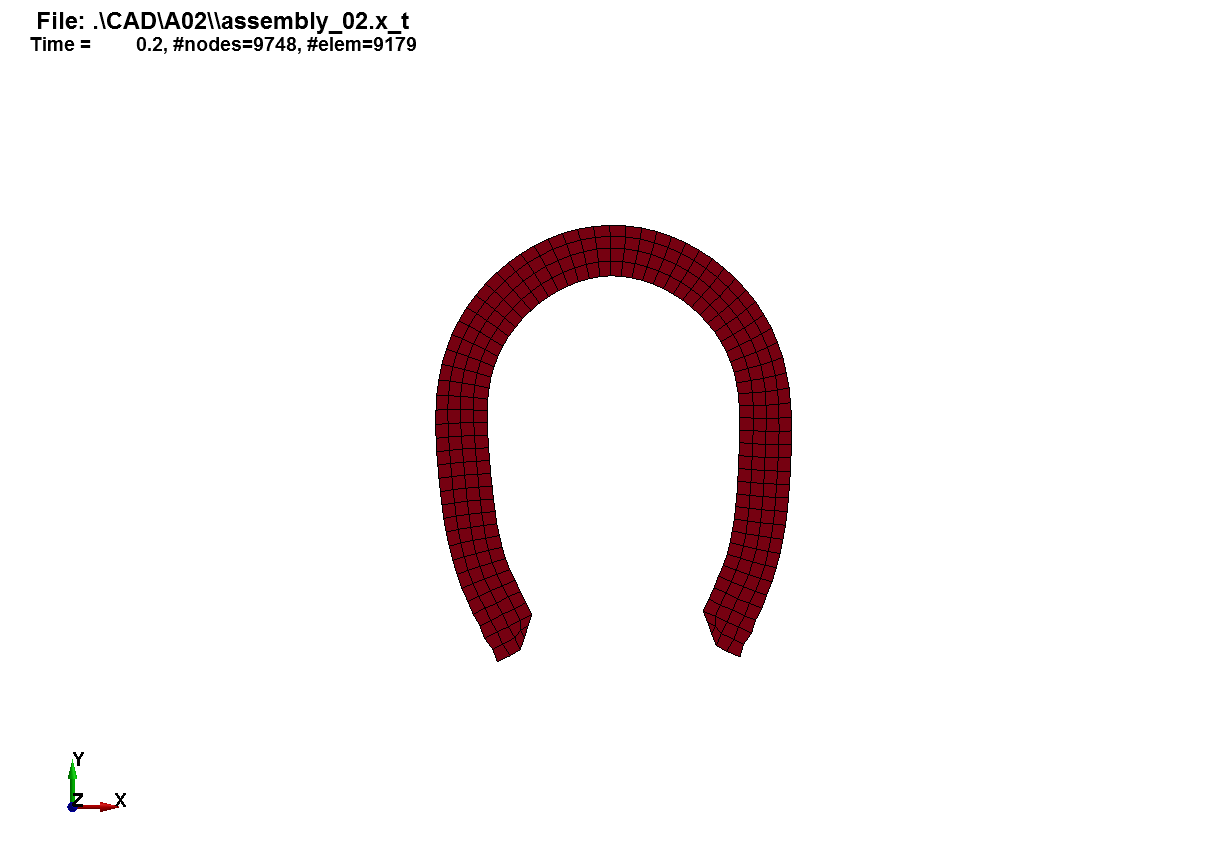
\includegraphics[width=0.75\textwidth]{src/ch4/geometry_01.png}
\captionof{figure}{Geometría resultante, primer paso}
\label{fig:geometry_01}
\end{center}

\begin{center}
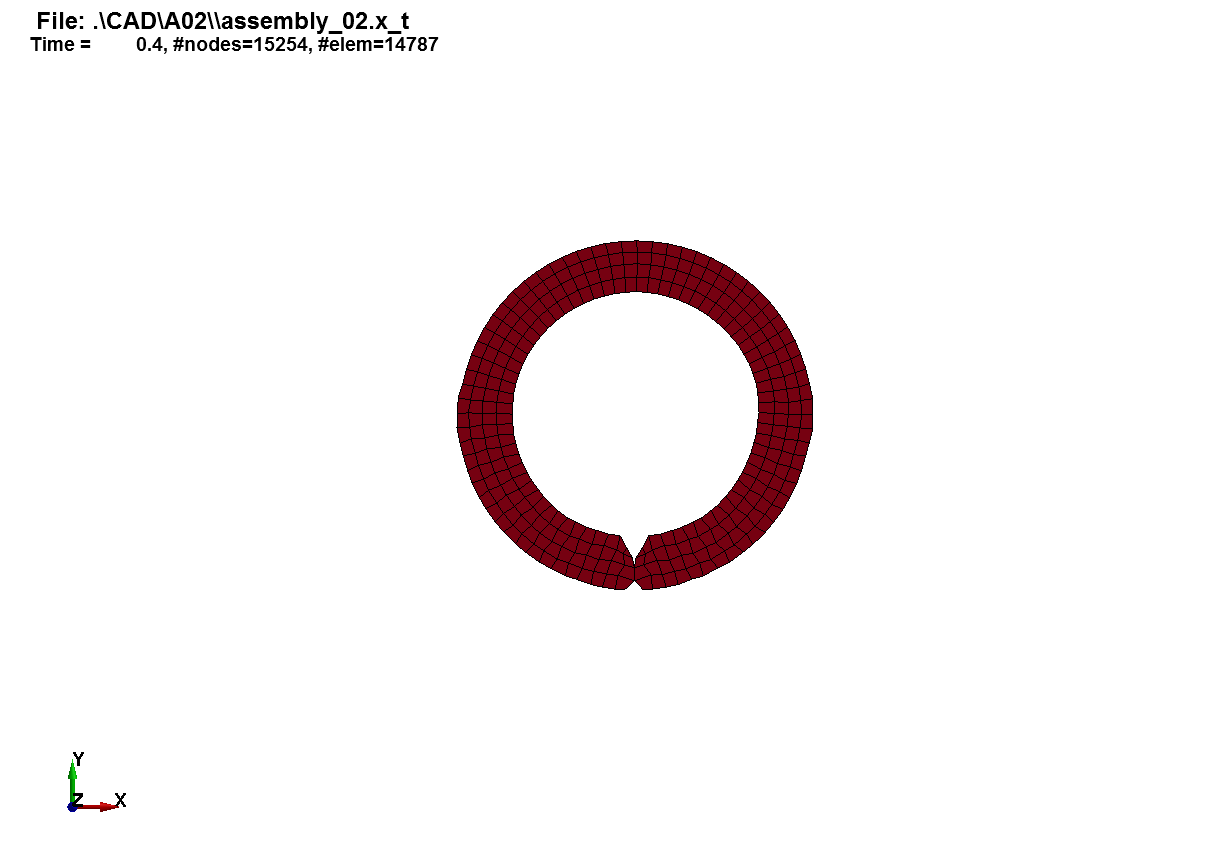
\includegraphics[width=0.75\textwidth]{src/ch4/geometry_02.png}
\captionof{figure}{Geometría resultante, segundo paso}
\label{fig:geometry_02}
\end{center}

La figura \ref{fig:thickness_variation} muestra una gráfica con las variaciones de espesor en la geometría 
final obtenida, las líneas punteadas corresponden a las tolerancias mínima y máxima del espesor. Para 
efectuar tal medición se tomaron como referencia nodos interiores y exteriores en la geometría final, 
posicionados sobre la misma vertical en la geometría inicial, y enseguida, basándose en las coordenadas 
iniciales y los desplazamientos, se obtuvo la distancia.

\begin{center}
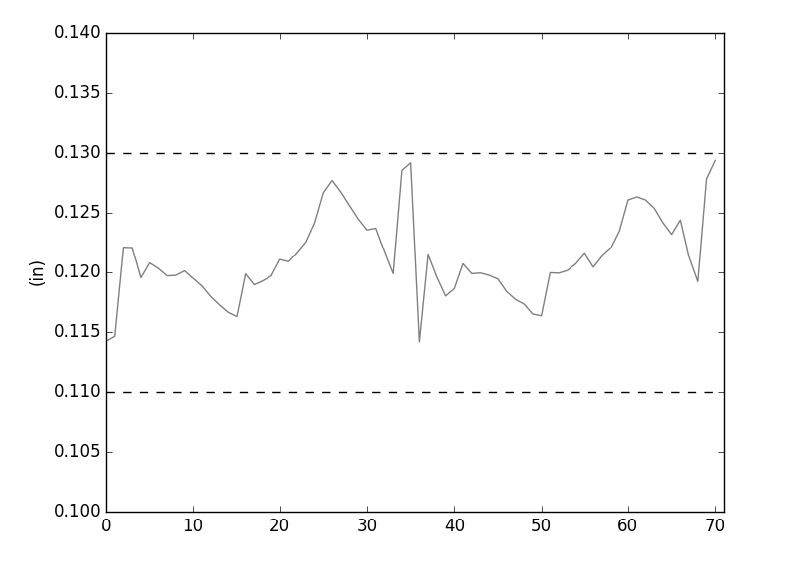
\includegraphics[width=0.75\textwidth]{src/ch4/thickness_variation.png}
\captionof{figure}{Variación del espesor de la geometría resultante}
\label{fig:thickness_variation}
\end{center}

\subsubsection{Esfuerzos}

La distribucíón de esfuerzos y sobre todo el historial del máximo se utilizó como 
un criterio comparativo  que aporta información acerca del estatus del material, 
es decir, para verificar que el material se encuentra en el rango de deformación 
plástica acorde a lo obtenido de forma experimental en la curva esfuerzo-deformación.\\

En las figuras \ref{fig:von_mises_01} y \ref{fig:von_mises_02} se muestran la 
distribución del esfuerzo de von Mises al final de la primer y segunda etapa 
del formado, respectivamente. 

\begin{center}
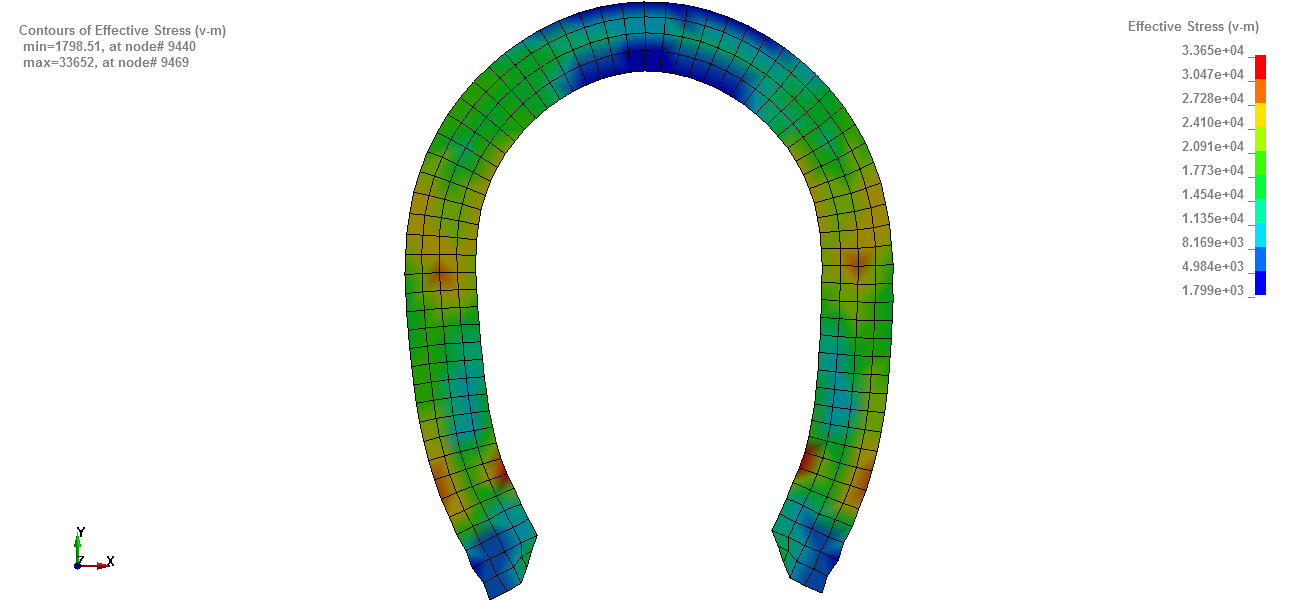
\includegraphics[width=0.75\textwidth]{src/ch4/von_mises_01.png}
\captionof{figure}{Distribución de esfuerzos de von Mises, final del primer paso, psi}
\label{fig:von_mises_01}
\end{center}

La figura \ref{fig:von_mises_stress_01} muestra la variación del esfuerzo máximo 
de von Mises para el primer paso de carga, cuyo valor máximo es de alrededor de 87,000 psi.

\begin{center}
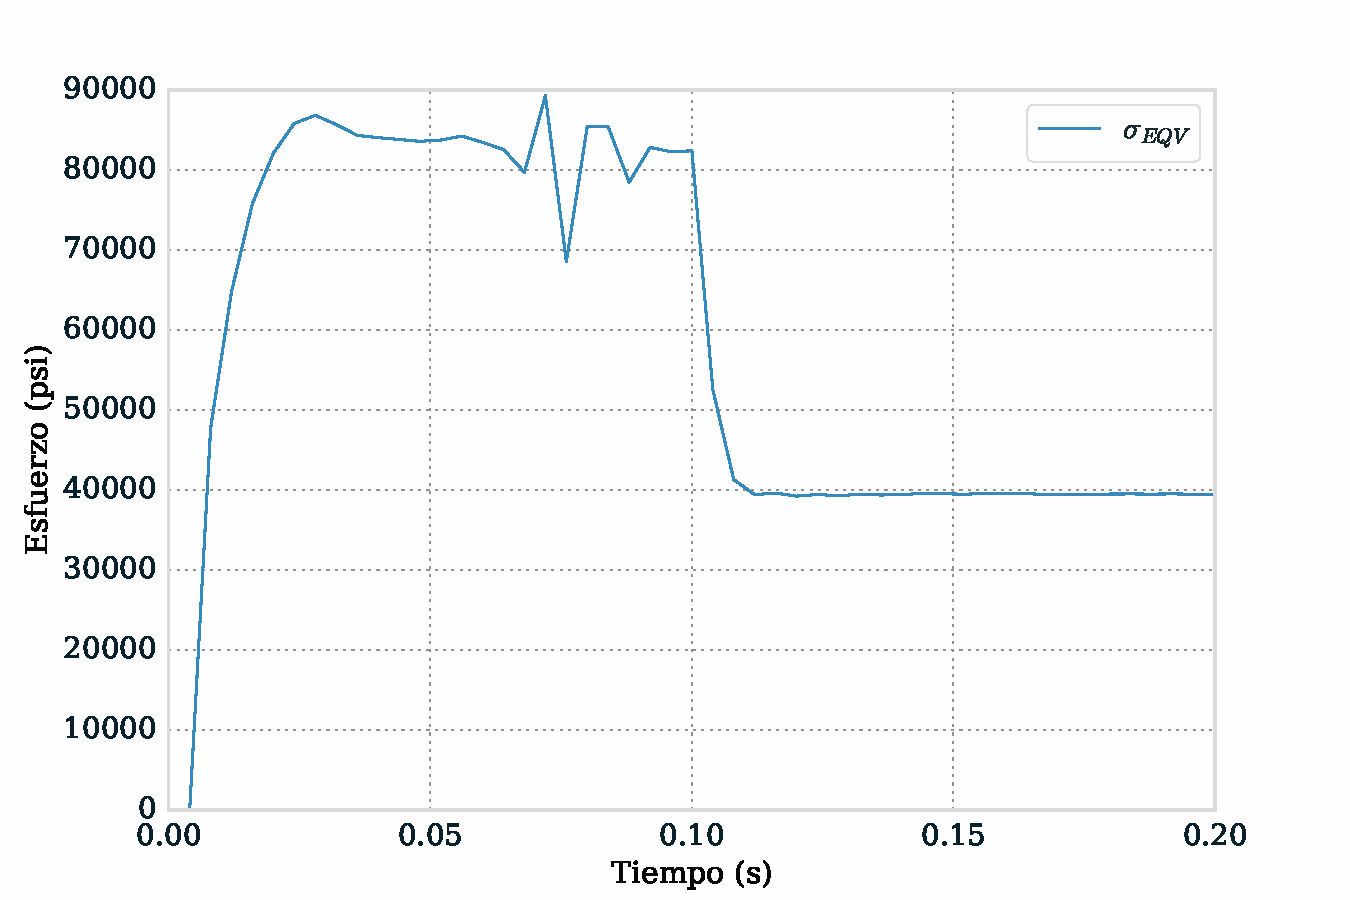
\includegraphics[width=0.75\textwidth]{src/ch4/von_mises_stress_01.pdf}
\captionof{figure}{Variación del esfuerzo máximo de von Mises}
\label{fig:von_mises_stress_01}
\end{center}

En \ref{fig:xyz_stress_01} se muestra el historial de esfuerzos en las direcciones 
X, Y, Z. Es evidente que el esfuerzo en dirección $Z$ es en general el menor de 
los tres, dado que este es calculado a partir de la ecuación de deformación plana 
que lo considera alrededor de una tercera parte de la suma de $\sigma_x$ y $\sigma_y$ para 
el caso de un acero. \\

\begin{center}
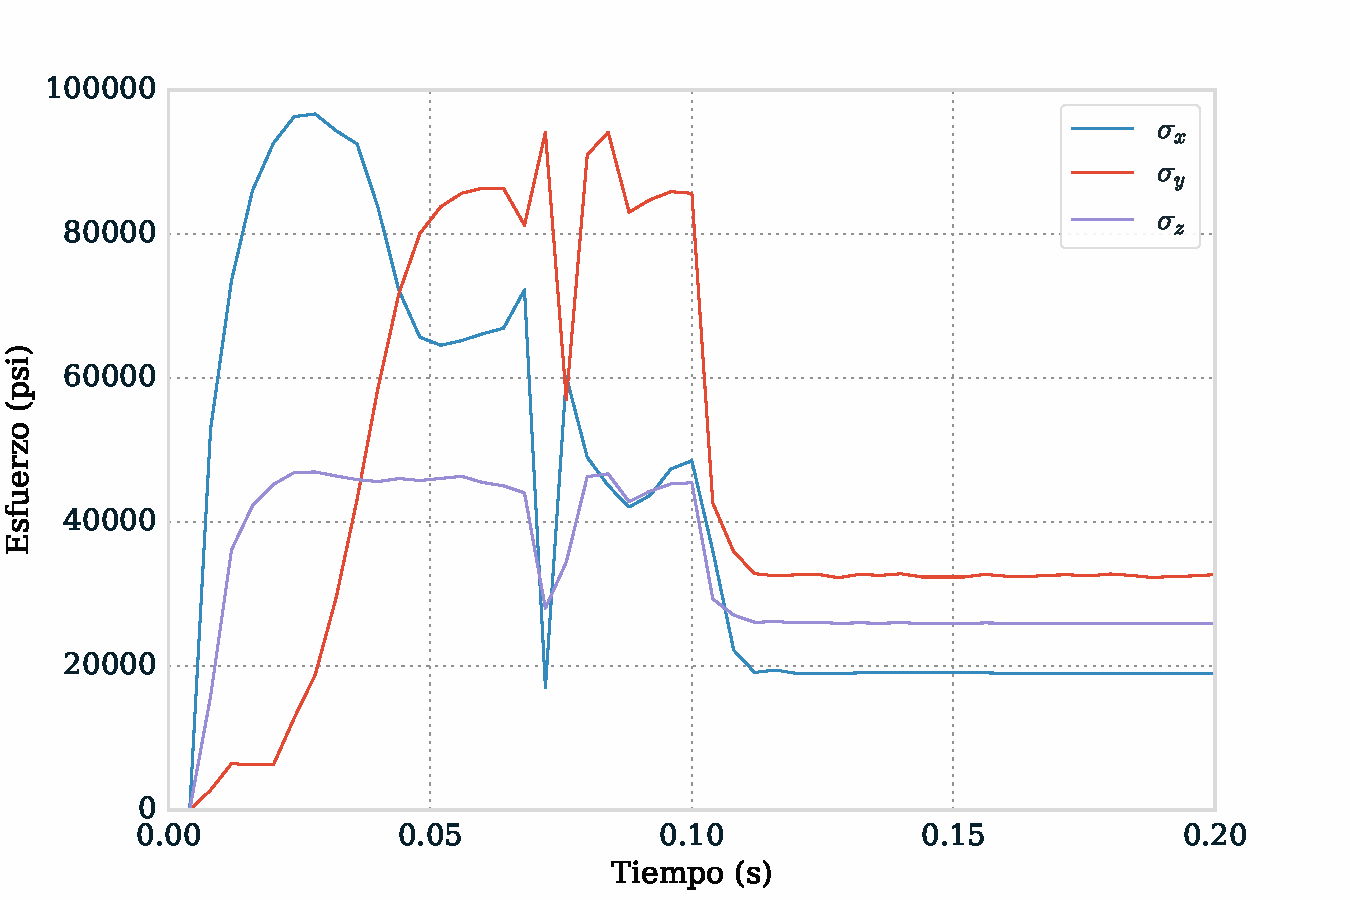
\includegraphics[width=0.75\textwidth]{src/ch4/xyz_stress_01.pdf}
\captionof{figure}{Variación de los esfuerzos máximos en dirección X,Y,Z}
\label{fig:xyz_stress_01}
\end{center}

\begin{center}
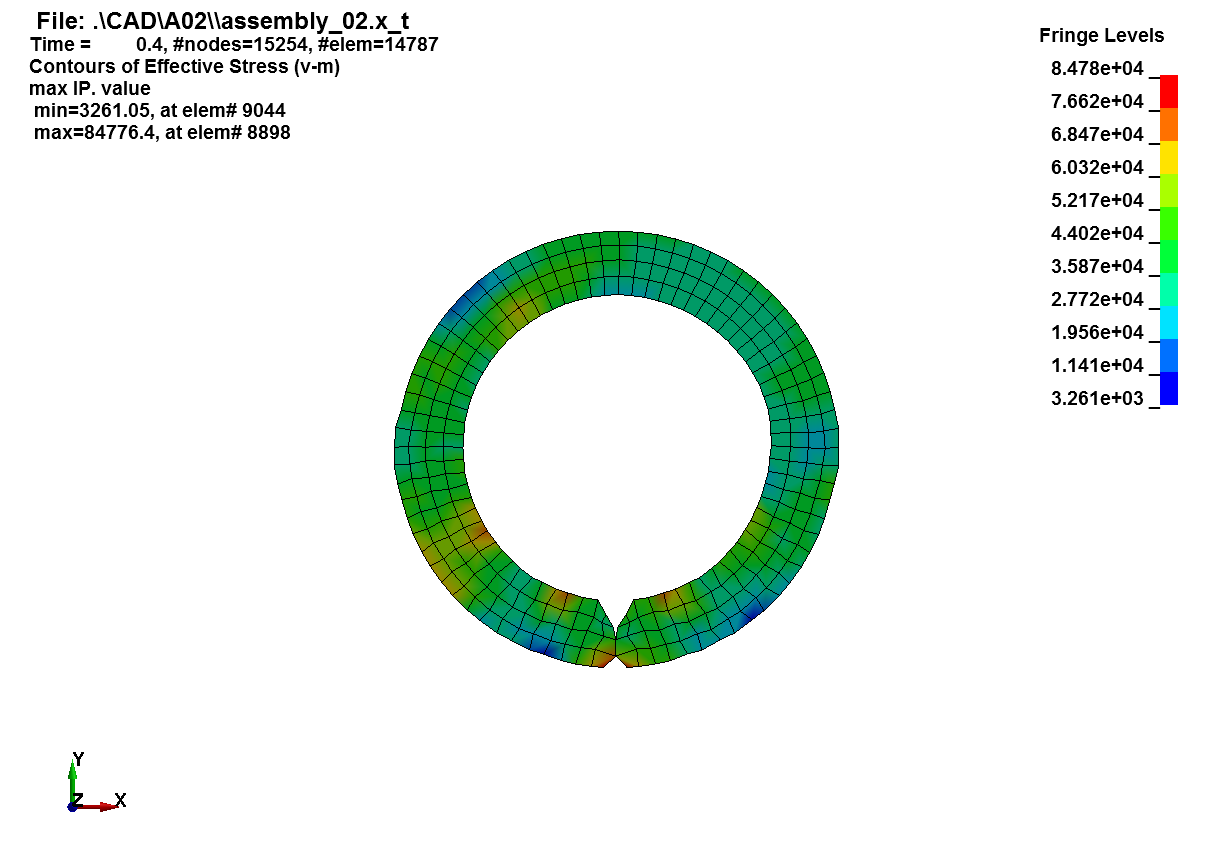
\includegraphics[width=0.75\textwidth]{src/ch4/von_mises_02.png}
\captionof{figure}{Distribución de esfuerzos de von Mises, final del segundo paso, psi}
\label{fig:von_mises_02}
\end{center}


\subsubsection{Deformaciones}

En las figuras \ref{fig:efective_plastic_strain_01} y \ref{fig:efective_plastic_strain_02} se muestran 
las distribuciones de la deformación plástica efectiva, al final de ambas etapas del formado. 

\begin{center}
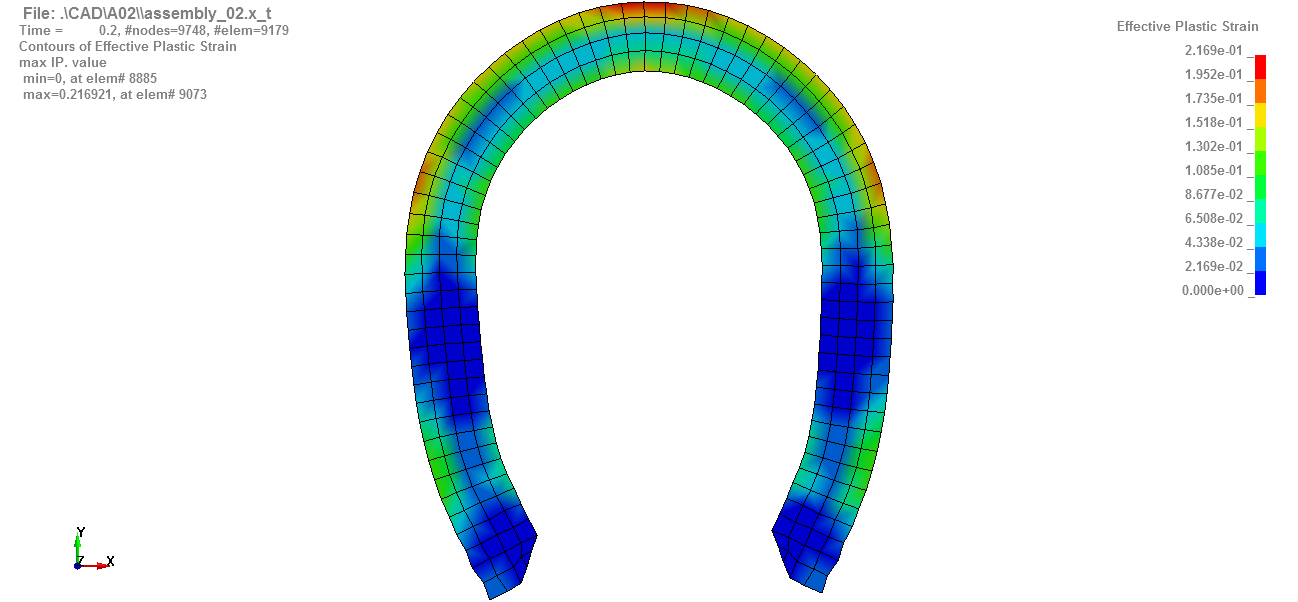
\includegraphics[width=0.75\textwidth]{src/ch4/efective_plastic_strain_01.png}
\captionof{figure}{Deformación plástica efectiva, final del primer paso}
\label{fig:efective_plastic_strain_01}
\end{center}

Tanto en \ref{fig:efective_plastic_strain_01} como en \ref{fig:efective_plastic_strain_02} se puede observar 
de manera clara una región intermedia que permanece con deformaciones muy pequeñas (región azul) o casi nulas, 
lo cual corresponde al eje neutro cuando se realiza una operación de doblado. Para una operación de doblado 
en donde el radio interior de doblado (0.285 in en este caso) es mayor al doble del espesor (0.12 in) se 
considera que el eje neutro se ubica alrededor de $0.42t$.

\begin{center}
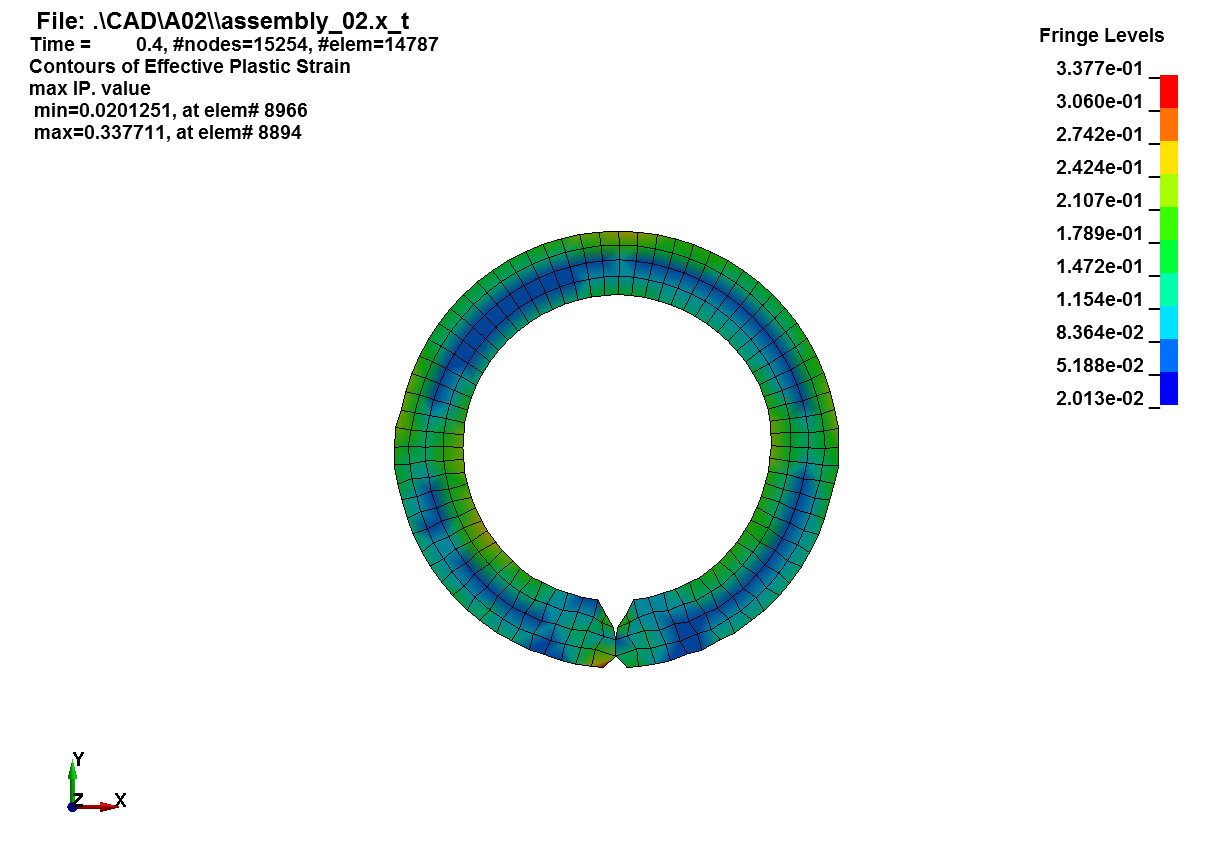
\includegraphics[width=0.75\textwidth]{src/ch4/efective_plastic_strain_02.png}
\captionof{figure}{Deformación plástica efectiva, final del segundo paso}
\label{fig:efective_plastic_strain_02}
\end{center}

% \begin{center}
% 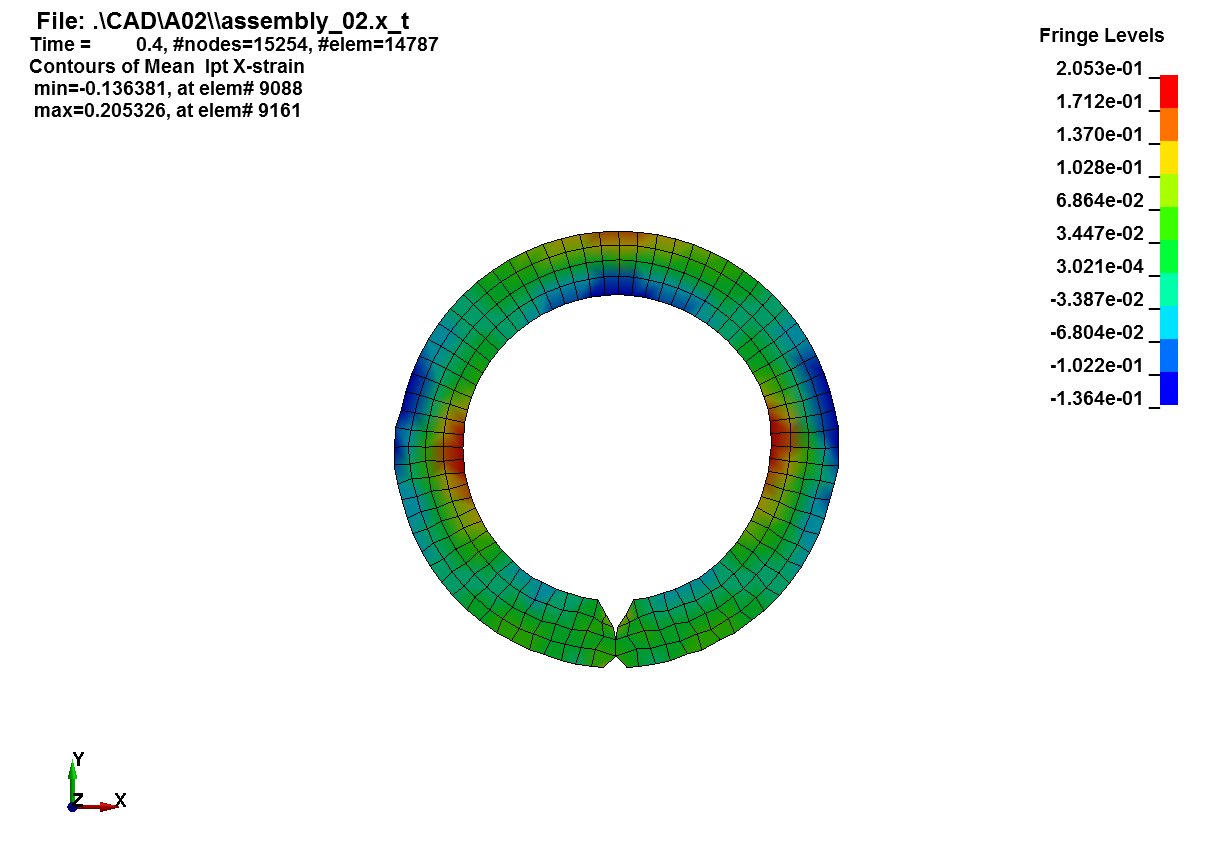
\includegraphics[width=0.75\textwidth]{src/ch4/strain_x_02.png}
% \captionof{figure}{Deformación en dirección X, final del segundo paso}
% \label{fig:efective_plastic_strain}
% \end{center}

% \begin{center}
% 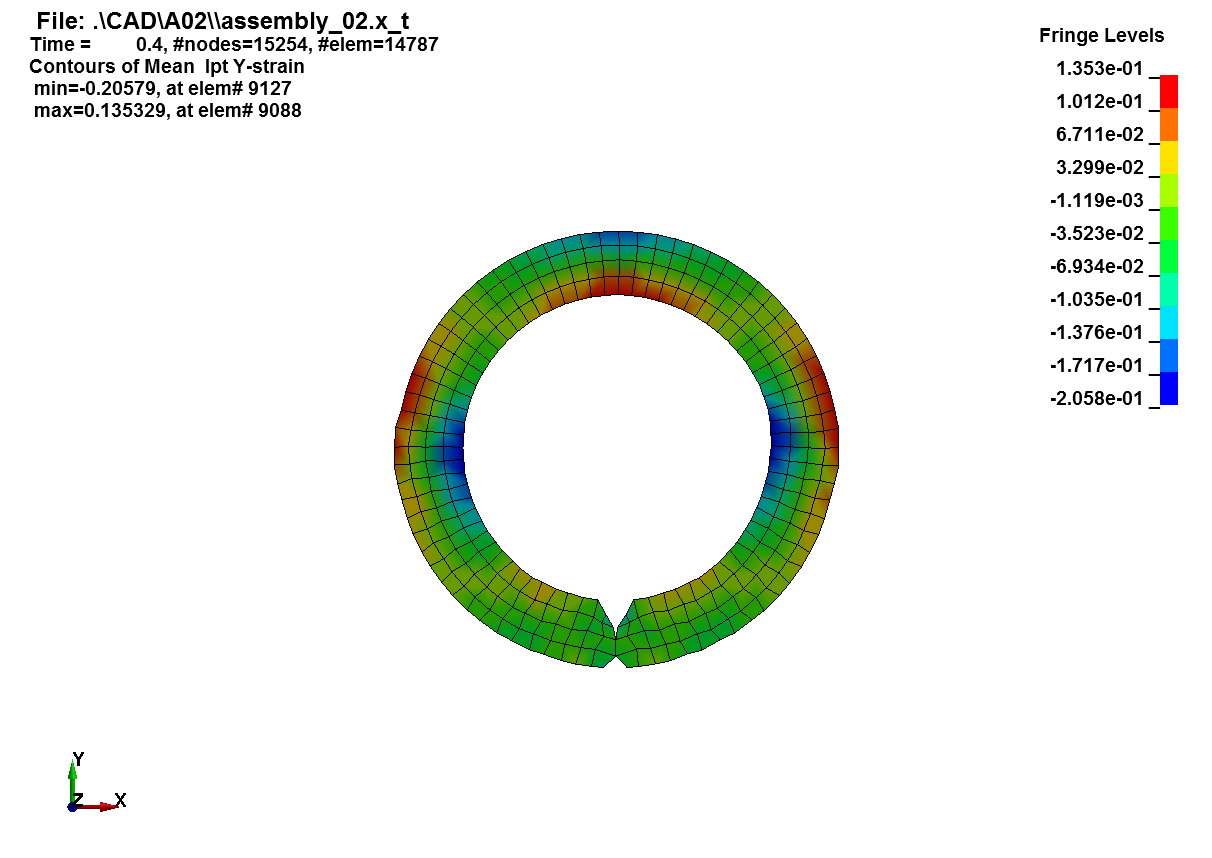
\includegraphics[width=0.75\textwidth]{src/ch4/strain_y_02.png}
% \captionof{figure}{Deformación en dirección Y, final del segundo paso}
% \label{fig:efective_plastic_strain}
% \end{center}


\subsubsection{Fuerza de formado}

En la figura \ref{fig:nodal_force_01} se puede observar que la fuerza máxima de formado 
requerida para completar el primer paso es de 2500 lbf, de donde se debe considerar 
que el análisis de deformación plana se realiza en base a una pieza de trabajo de 
ancho unitario. Este resultado se puede extrapolar a la pieza real si multiplicamos el 
resultado por un factor de 3 que es lo correspondiente a la longitud del \textit{blank}, 
por tanto la fuerza requerida correspondería a 7500 lbf.\\

De la gráfica de \ref{fig:nodal_force_01} se puede observar también que existen dos máximos 
locales correspondientes a la fuerza requerida para la operación de los formadores superiores y 
de las levas formadoras, de manera respectiva.\\

El primer máximo local, que corresponde al doblado realizado por los formadores, se puede 
comparar con la fuerza calculada de manera analítica a partir de la ecuación \ref{eq:fuerza_doblado}, 
de la cual se tiene:

$$
F = \frac{K S_{t} w t^2}{D} = \frac{(1.33)(52000)(3)(0.12)^2}{0.93} = 3212 \text{lbf}
$$

El resultado de la fuerza de formado obtenida mediante la simulación corresponde a un valor de 
3600 lbf, lo cual implica una diferencia o error relativo de 10\% de sobrestimación mediante 
el análisis numérico.

\begin{center}
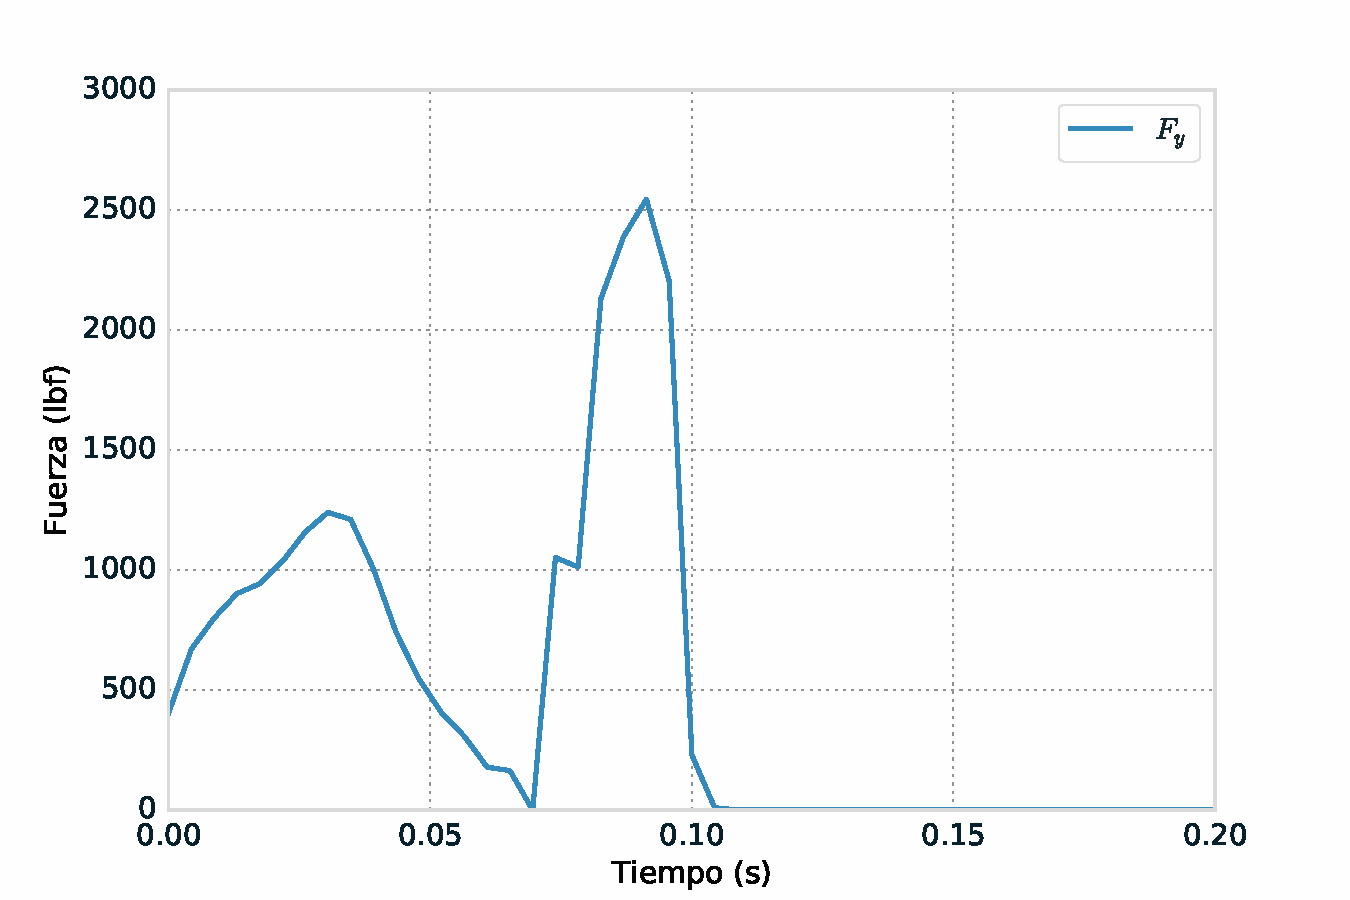
\includegraphics[width=0.75\textwidth]{src/ch4/nodal_force_01.pdf}
\captionof{figure}{Fuerza de formado requerida, primer paso}
\label{fig:nodal_force_01}
\end{center}

En la figura \ref{fig:nodal_force_02} se muestra la fuerza de formado requerida para completar el 
segundo paso del formado, misma que se calculó en alrededor de 90,000 lbf (40.8 ton). En este punto 
hay que considerar que la fuerza requerida varía considerablemente dependiendo del desplazamiento 
del formador superior, y de esto depende, la forma final del tubo obtenido, con lo aquí descrito se 
obtuvo una geometría como la mostrada en \ref{fig:geometry_02}.

\begin{center}
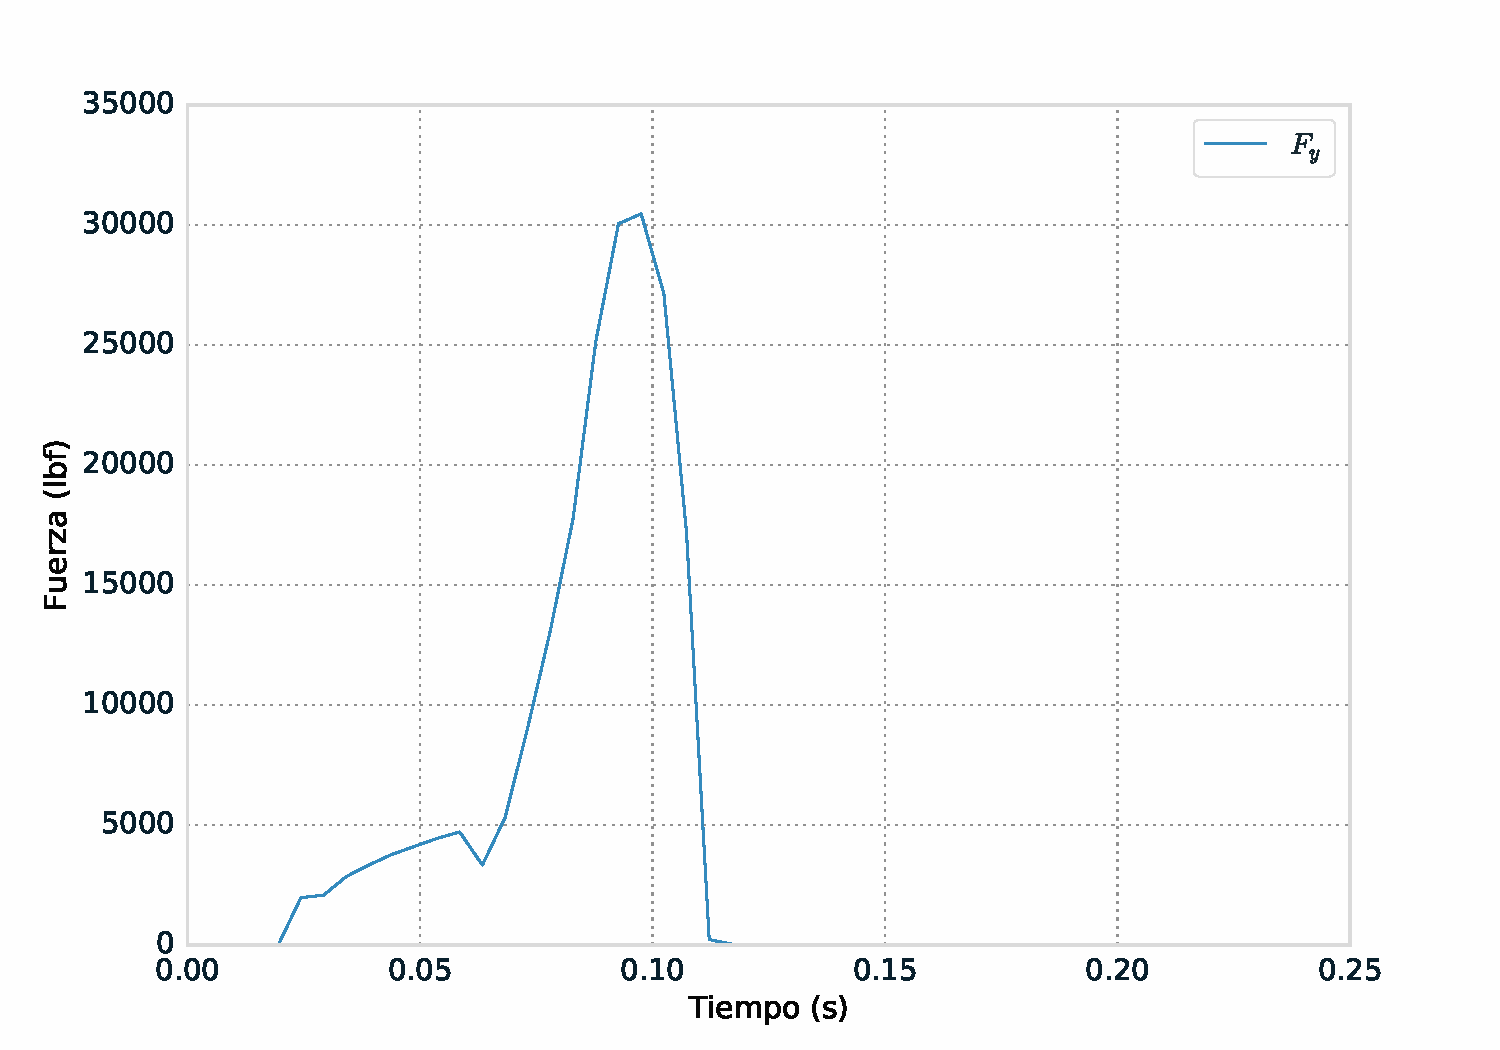
\includegraphics[width=0.75\textwidth]{src/ch4/nodal_force_02.pdf}
\captionof{figure}{Fuerza de formado requerida, segundo paso}
\label{fig:nodal_force_02}
\end{center}

\subsubsection{Influencia del escalamiento de masa}\label{sec:mass-scaling-results}

En la sección \ref{sec:mass-scaling} se describió el proceso para utilizar el escalamiento de masa 
selectivo en un análisis de tipo dinámico explícito, cuyo objetivo es reducir el tiempo de 
solución de una simulación mediante la introducción controlada de \textit{masa artificial} que implica 
un aumento en la densidad del material y esto a su vez la reducción de los intervalos de tiempo.\\

Para evidenciar lo comentado en el párrafo anterior, en lo subsiguiente se presenta el análisis de cinco simulaciones realizadas con escalamientos de 
masa selectivo, en donde el tamaño mínimo del paso de tiempo se varía desde $1x10^{-7}$ hasta 
$5x10^{-7}$.\\

La figura \ref{fig:ms_sol_time} muestra la variación del tiempo de solución (CPU Time) comparado con 
el porcentaje de masa agregado. Se observa que la curva resultante muestra el comportamiento de 
una función exponencial decreciente y que con un 12\% de masa adicional se puede reducir el tiempo 
de solución hasta un 30\% respecto al tiempo de solución sin escalamiento de masa.

\begin{center}
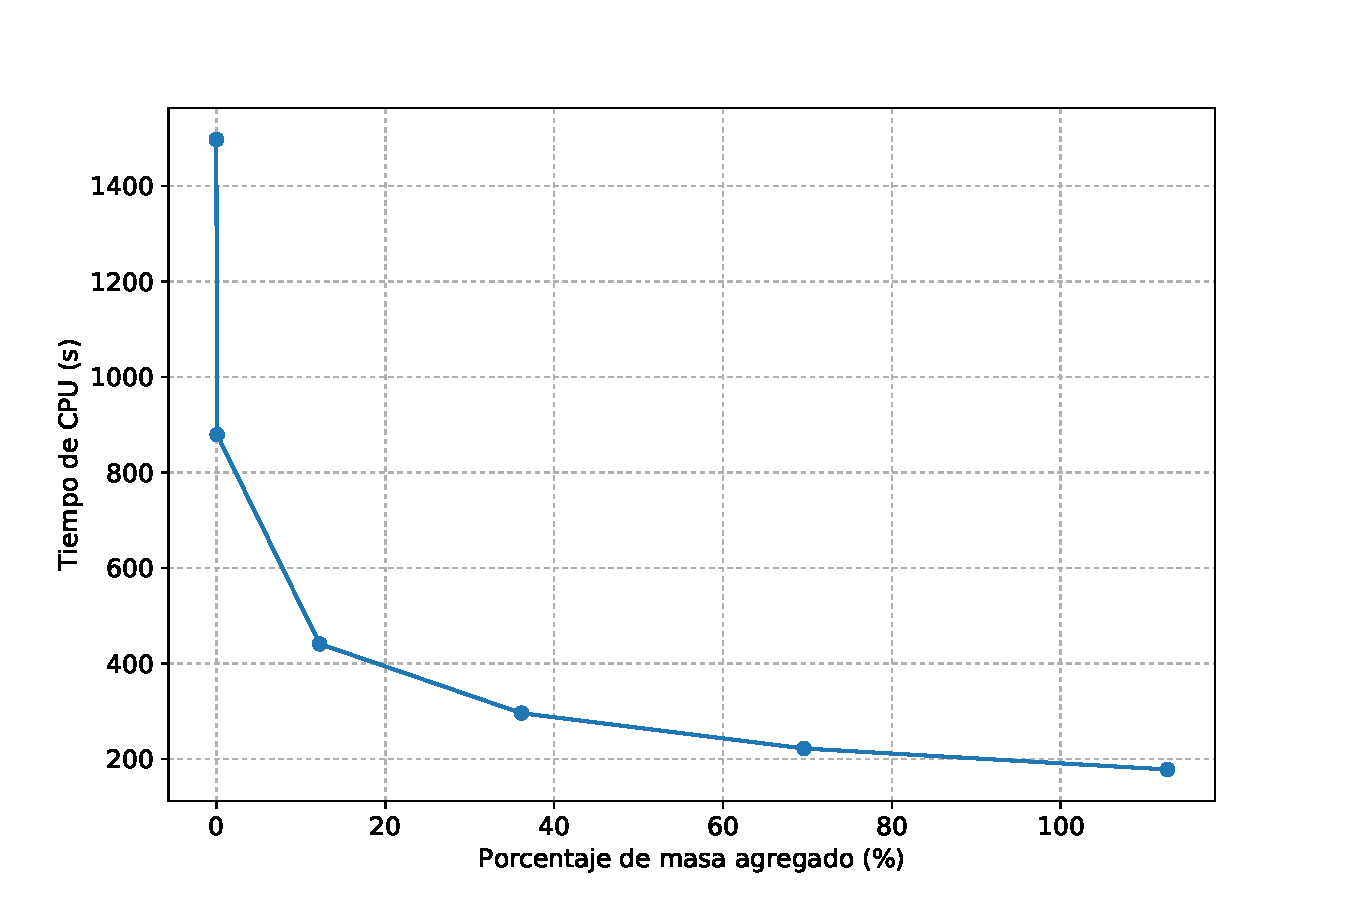
\includegraphics[width=0.75\textwidth]{src/ch4/ms_sol_time.pdf}
\captionof{figure}{Tiempo de solución para diversos escalamientos de masa}
\label{fig:ms_sol_time}
\end{center}

En la figura \ref{fig:ms_von_mises} se muestra la variación del esfuerzo equivalente máximo de von Mises, cuando 
se aplica el escalamiento de masa. Se puede observar que la variación entre cada uno de los casos 
es mínima en todo el historial de tiempo, habiendo una diferencia significativa en el tiempo 
correspondiente a cuando los formadores superiores dejan de actuar y las levas aún no interactúan 
con la pieza de trabajo.

\begin{center}
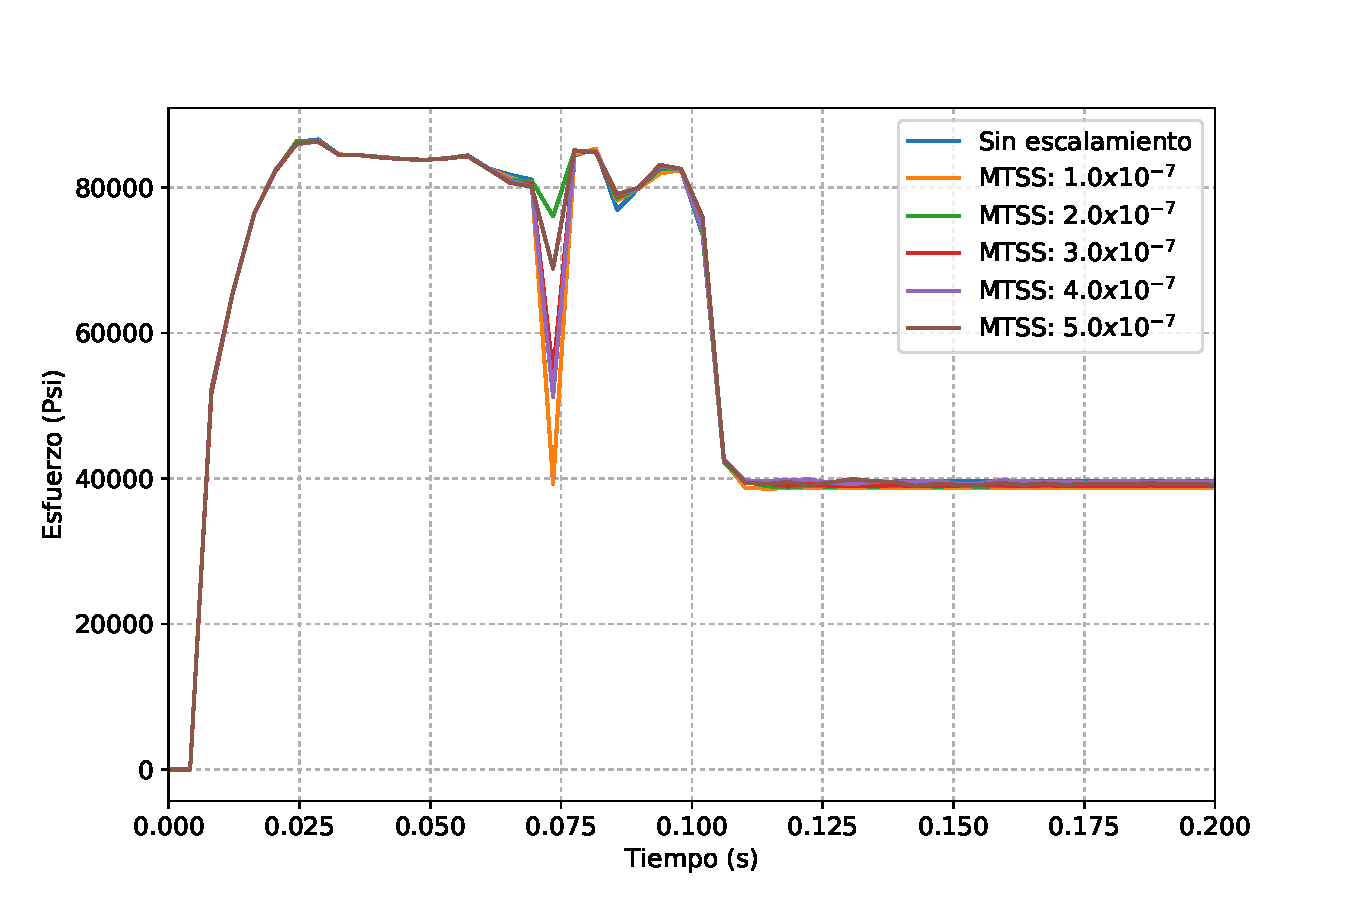
\includegraphics[width=0.75\textwidth]{src/ch4/ms_von_mises.pdf}
\captionof{figure}{Variación del esfuerzo de von Mises utilizando escalamiento de masa}
\label{fig:ms_von_mises}
\end{center}

En \ref{fig:ms_force} se muestra la variación de la fuerza de formado, se observa que el 
comportamiento es prácticamente similar para todos los casos.

\begin{center}
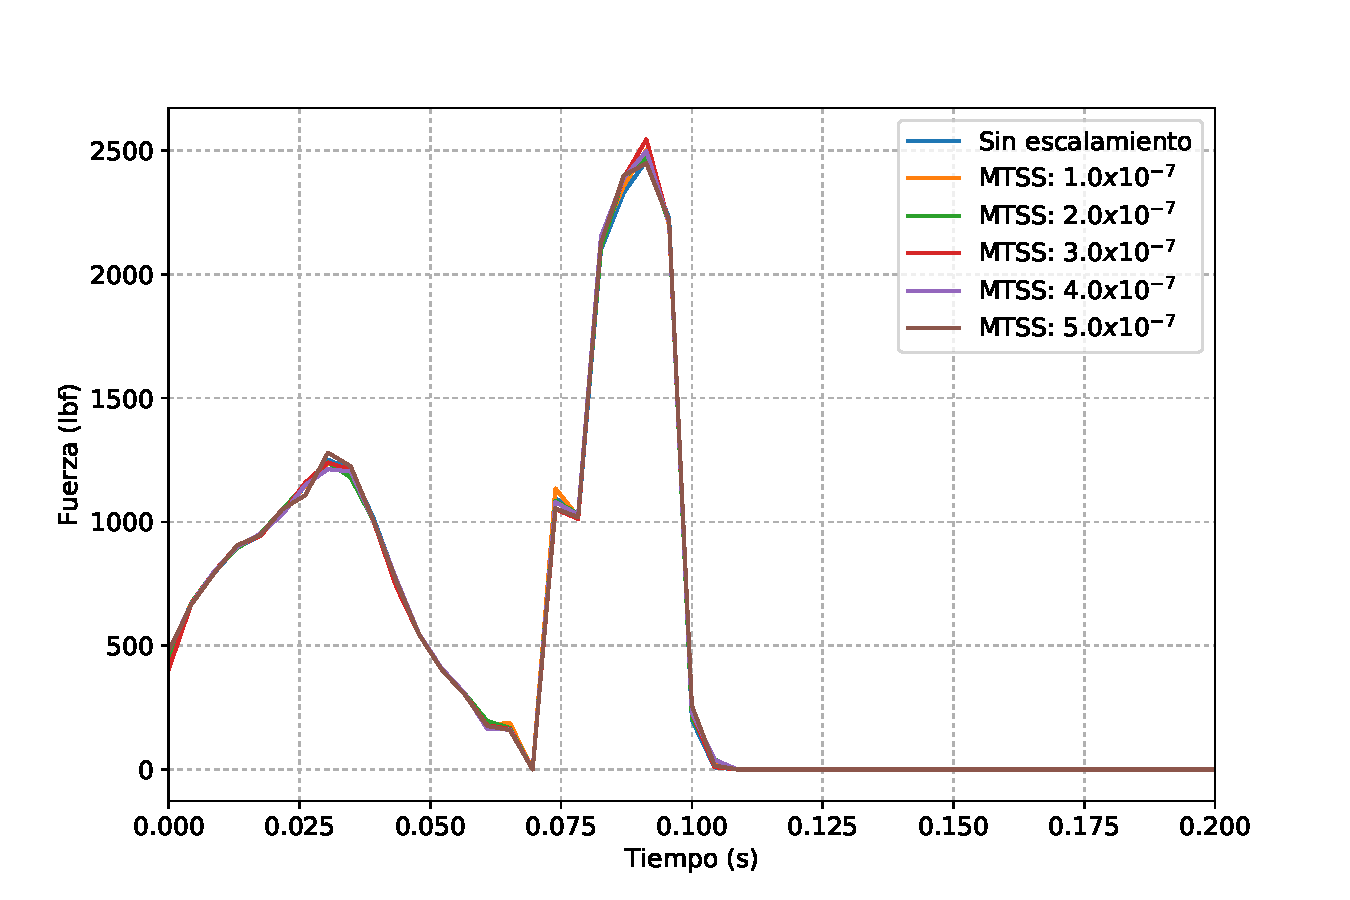
\includegraphics[width=0.75\textwidth]{src/ch4/ms_force.pdf}
\captionof{figure}{Variación de la fuerza de formado usando escalamiento de masa}
\label{fig:ms_force}
\end{center}

Con lo observado, se puede asumir que la influencia del escalamiento de masa, agregando hasta alrededor 
de un 110\% de masa, no es significativa, y permite reducir hasta en un 90\% el tiempo de solución de 
un análisis dinámico-explícito, lo cual representa una enorme ventaja.\\

\textbf{Escalamiento de masa excesivo} \\

Un escalamiento de masa excesivo normalmente conlleva a un resultado alejado de la realidad, las formas 
geométricas deformadas tienden a no corresponder con lo esperado, debido a que los efectos de la inercia 
inducida por la introducción de masa artificial son muy exagerados. Por ejemplo, en la figura 
\ref{fig:ms_excessive} se muestra una simulación que resulta de utilizar un escalamiento de masa bastante 
exagerado (un proporción mayor a 400 de \textit{masa agregada}); se puede observar claramente que la geometría 
de la pieza de trabajo se deforma hasta una configuración improbable para un material rígido como el acero, 
aún cuando los formadores superiores no están en contacto directo en ese instante, esto debido a que la 
energía cinética (que aumenta con la masa) del modelo representa una fracción superior al 10\% de la 
energía interna.\\

\begin{center}
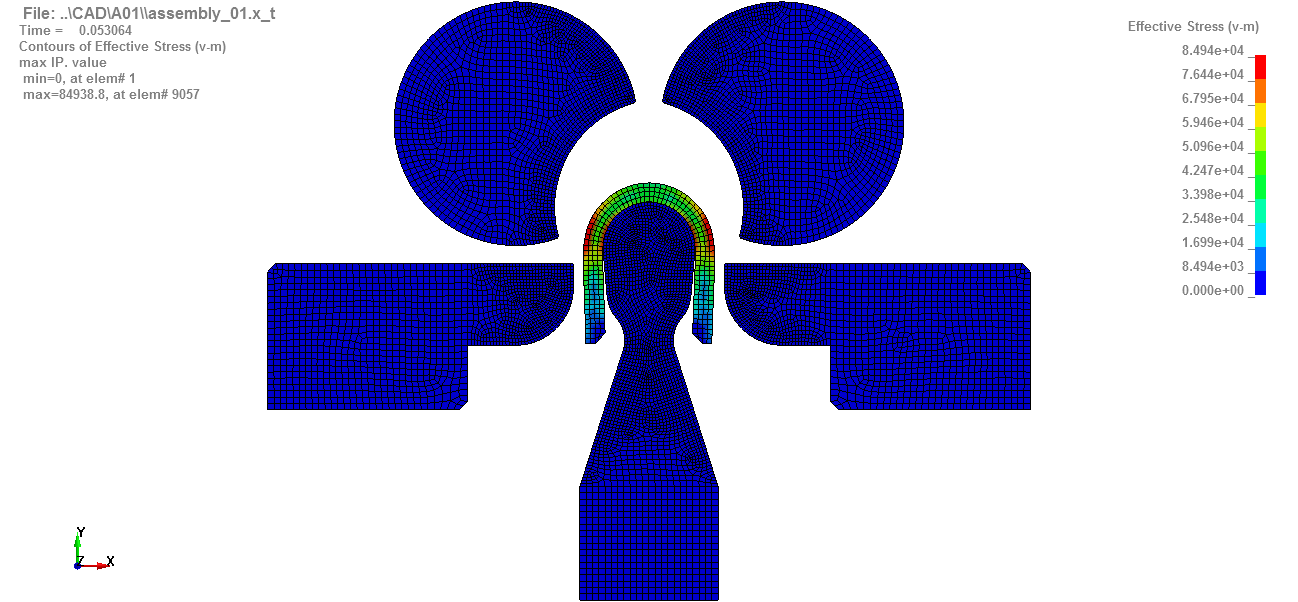
\includegraphics[width=0.85\textwidth]{src/ch4/ms_excessive.png}
\captionof{figure}{Algunos efectos del escalamiento excesivo de masa}
\label{fig:ms_excessive}
\end{center}

\subsubsection{Modelos de material}

En las figuras  \ref{fig:mdm_von_mises} y \ref{fig:mdm_force} se muestran las gráficas correspondientes 
al esfuerzo máximo de von Mises y la fuerza de formado, respectivamente, de la evaluación de los diversos 
modelos de material que ahí se listan.\\

Tanto la variación de los esfuerzos, como la de la fuerza de formado, es poco significativa, mostrando 
un comportamiento similar en ambos casos para todos los modelos de material utilizados. La 
diferencia más notoria ocurre en los esfuerzos residuales que quedan al finalizar el proceso 
de formado, en donde se observa una diferencia de alrededor de un 20\% del modelo multilineal 
respecto al bilineal cinemático.

\begin{center}
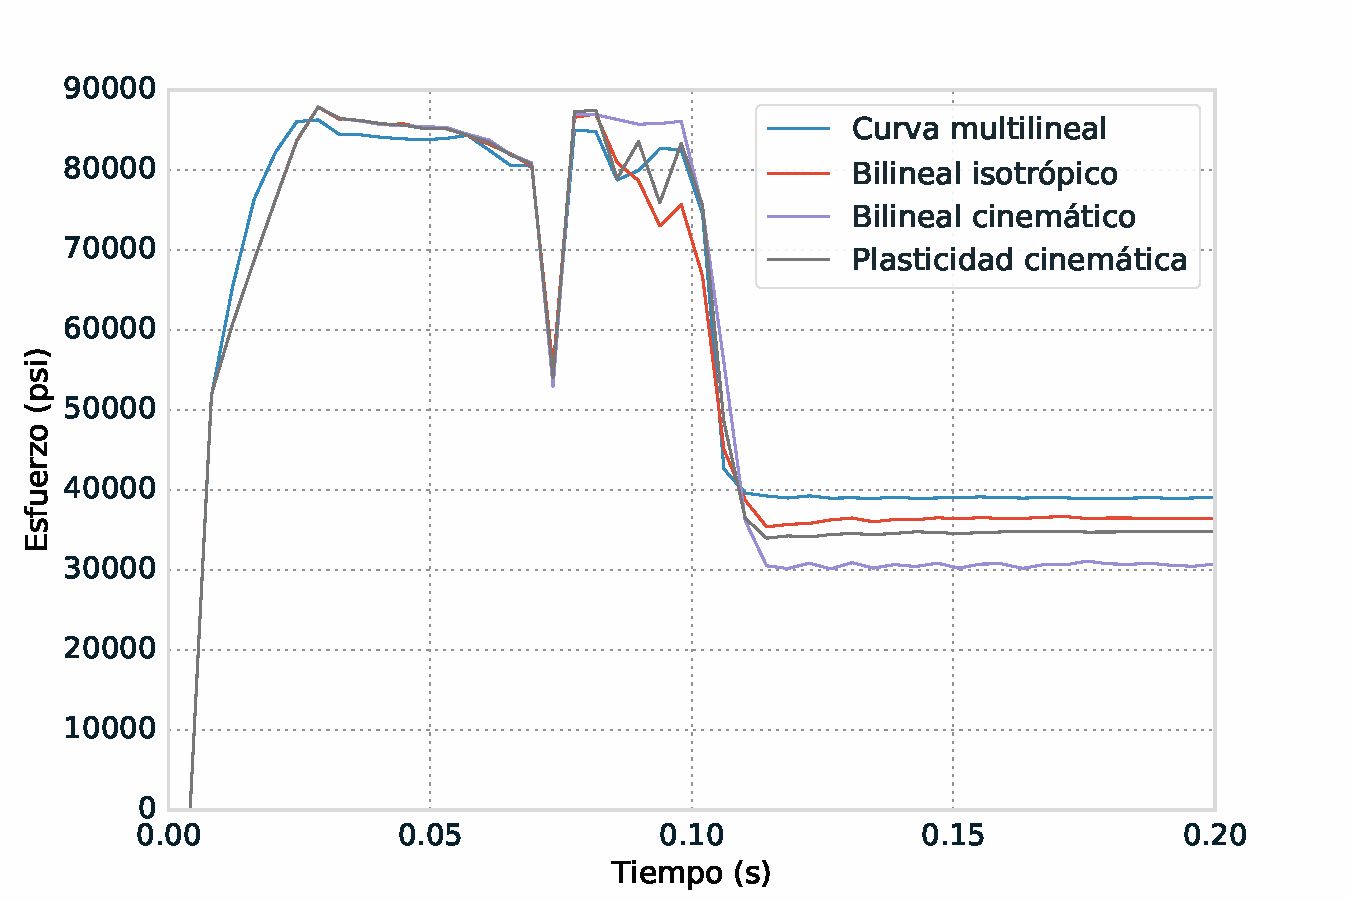
\includegraphics[width=0.75\textwidth]{src/ch4/mdm_von_mises.pdf}
\captionof{figure}{Variación del esfuerzo de von Mises para diversos modelos constitutivos}
\label{fig:mdm_von_mises}
\end{center}

\begin{center}
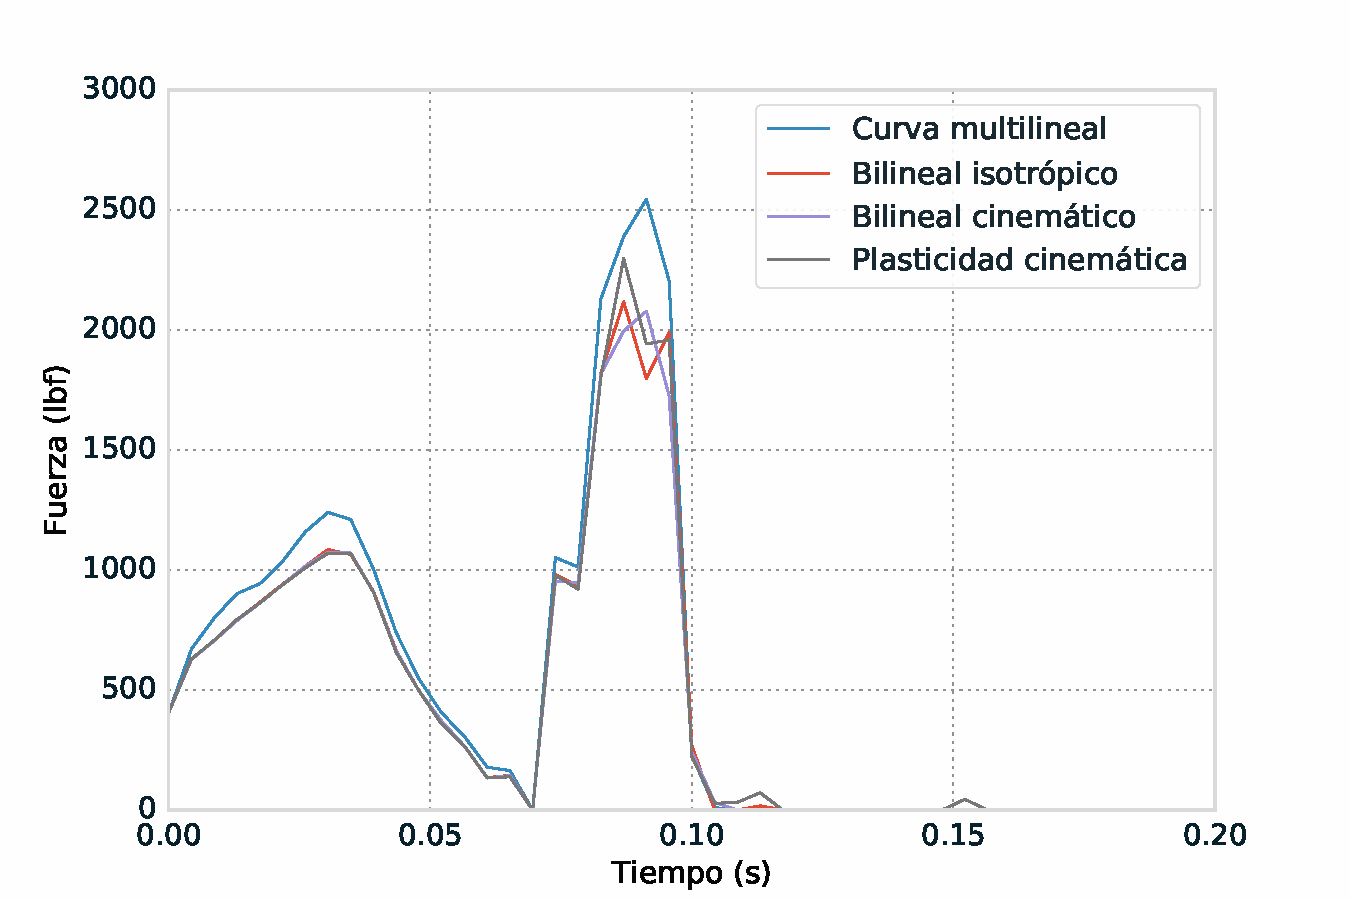
\includegraphics[width=0.75\textwidth]{src/ch4/mdm_force.pdf}
\captionof{figure}{Variación de la fuerza de formado para diversos modelos constitutivos}
\label{fig:mdm_force}
\end{center}

\subsection{Análisis 3D}

En lo subsiguiente se muestran los resultados obtenidos para el análisis tridimensional 
realizado. Se omite el análisis de energía realizado para el caso bidimensional, además 
de lo correspondiente al modo de deformación de Hourglass, puesto que en este caso el 
elemento \texttt{SOLID164} utilizado es un elemento de tipo \textit{full integration} y 
no presenta problemas de este tipo.

\subsubsection{Esfuerzos}

En las figuras \ref{fig:von_mises_3D_01} y \ref{fig:von_mises_3D_01} se muestra la distribución 
de esfuerzos al final del primer y segundo paso del formado, además de las geometrías 
resultantes en ambos casos.\\

En \ref{fig:von_mises_3d_all} se muestra la variación del esfuerzo de von Mises máximo en 
el historial de tiempo, para ambas etapas del formado.

\begin{center}
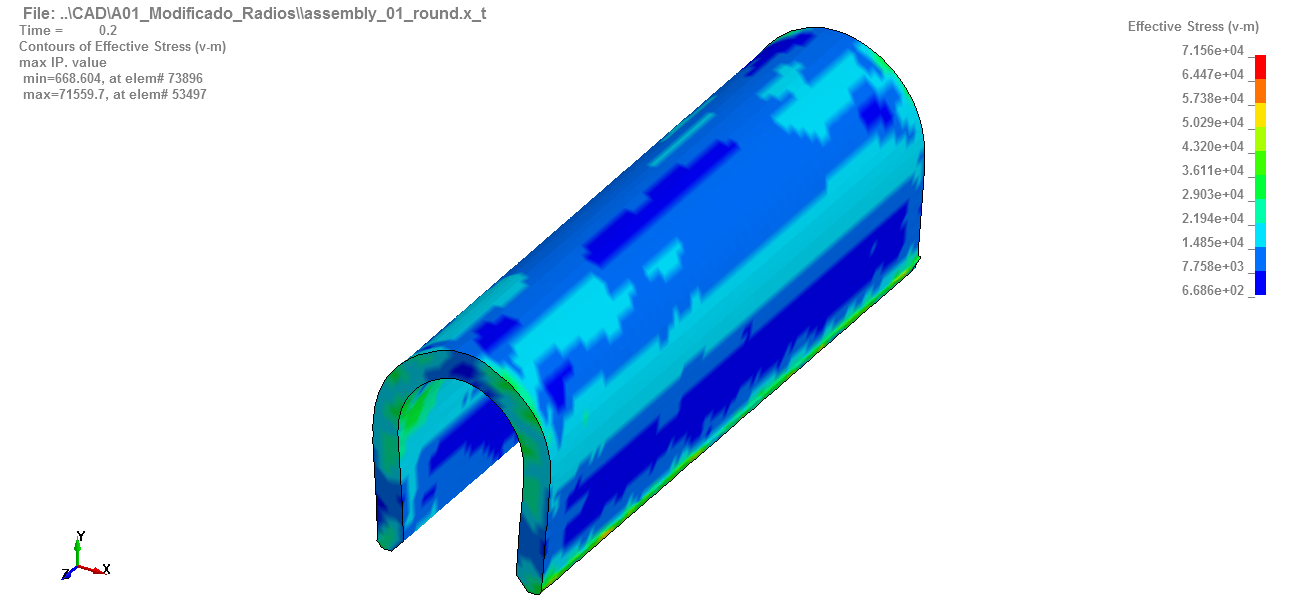
\includegraphics[width=0.75\textwidth]{src/ch4/von_mises_3D_01.png}
\captionof{figure}{Distribución del esfuerzo de von Mises}
\label{fig:von_mises_3D_01}
\end{center}

\begin{center}
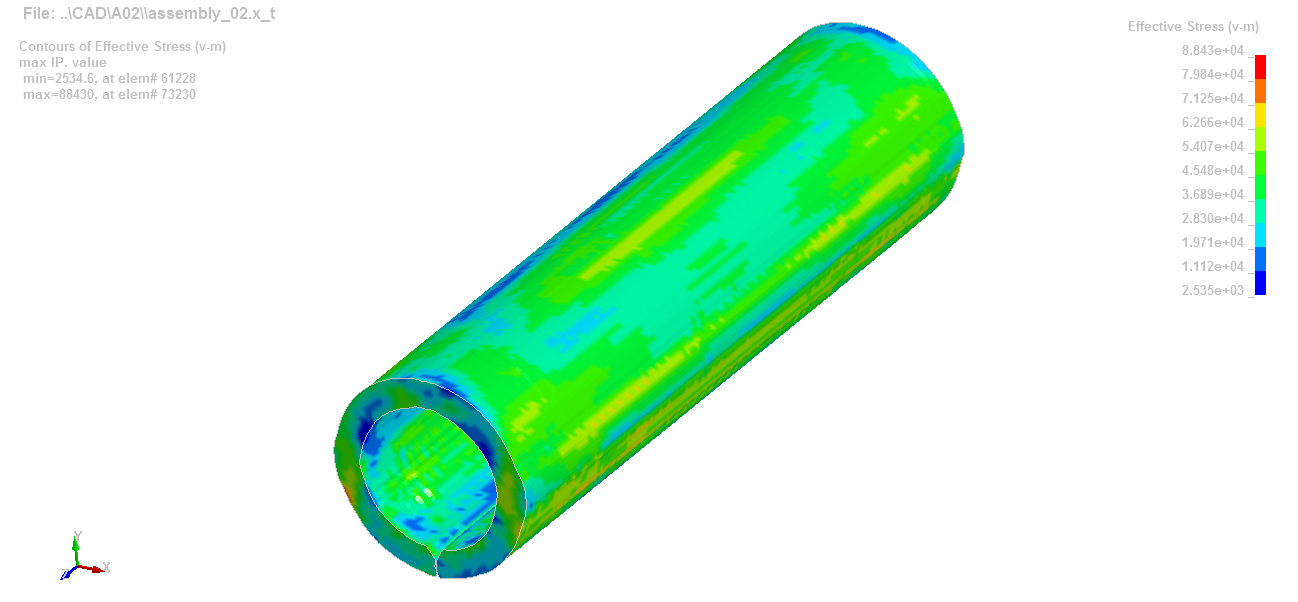
\includegraphics[width=0.75\textwidth]{src/ch4/von_mises_3D_02.png}
\captionof{figure}{Distribución del esfuerzo de von Mises, segundo paso}
\label{fig:von_mises_3D_02}
\end{center}

\begin{center}
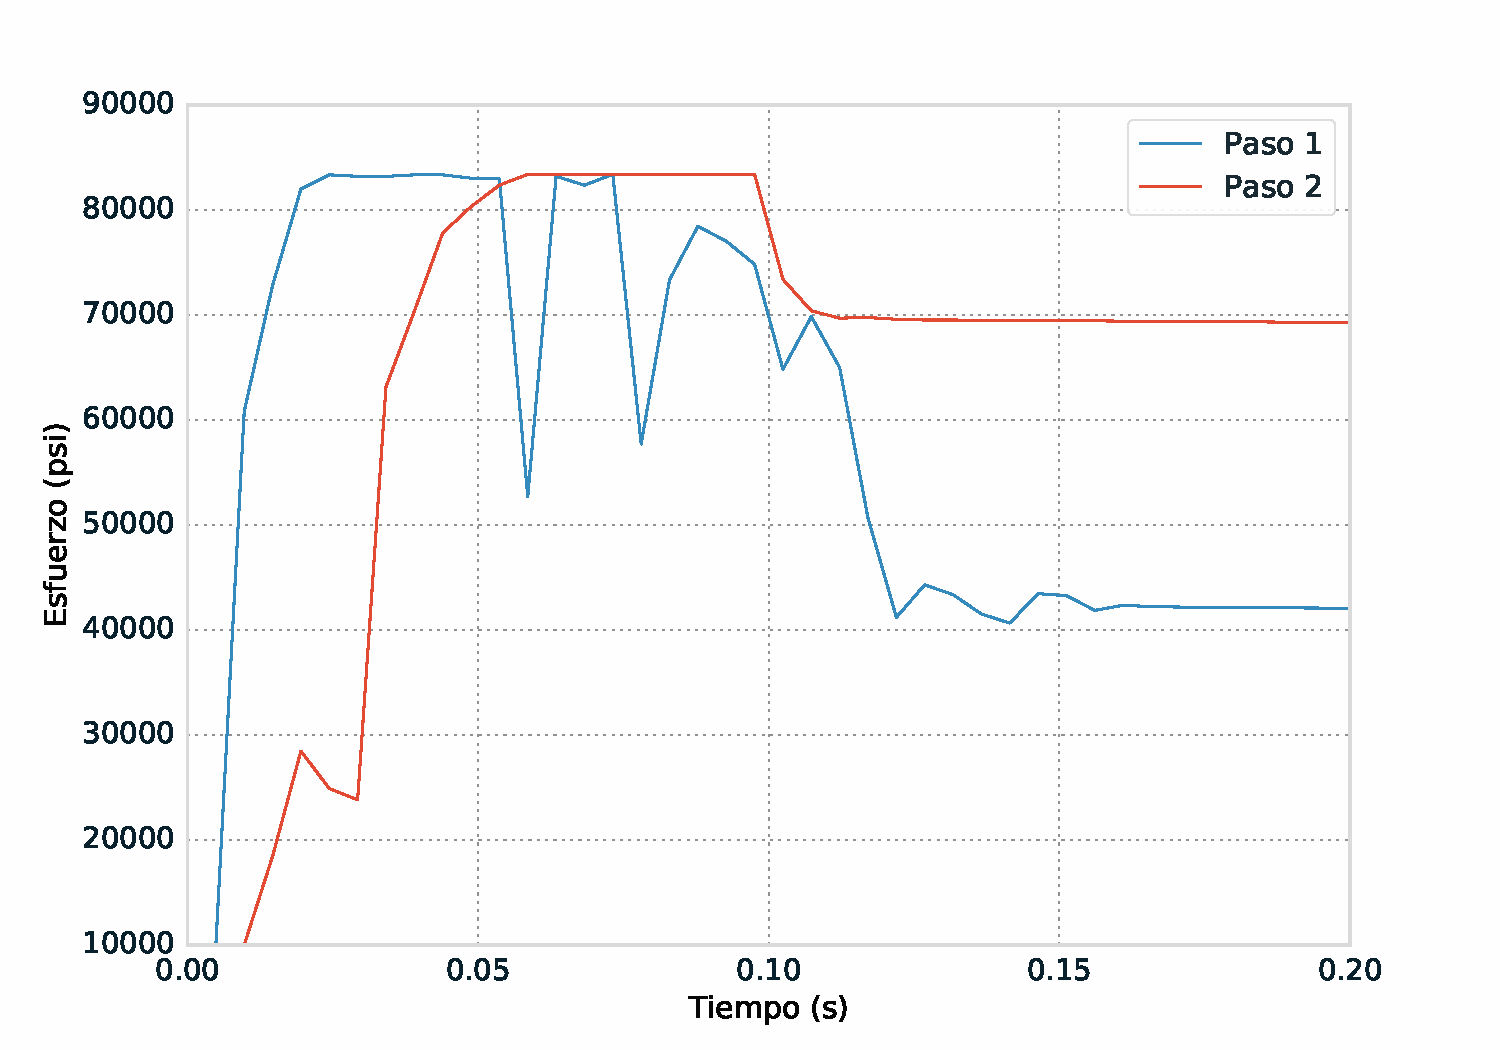
\includegraphics[width=0.75\textwidth]{src/ch4/von_mises_3d_all.pdf}
\captionof{figure}{Variación del esfuerzo máximo de von Mises}
\label{fig:von_mises_3d_all}
\end{center}

% \subsubsection{Deformaciones}

% \begin{center}
% 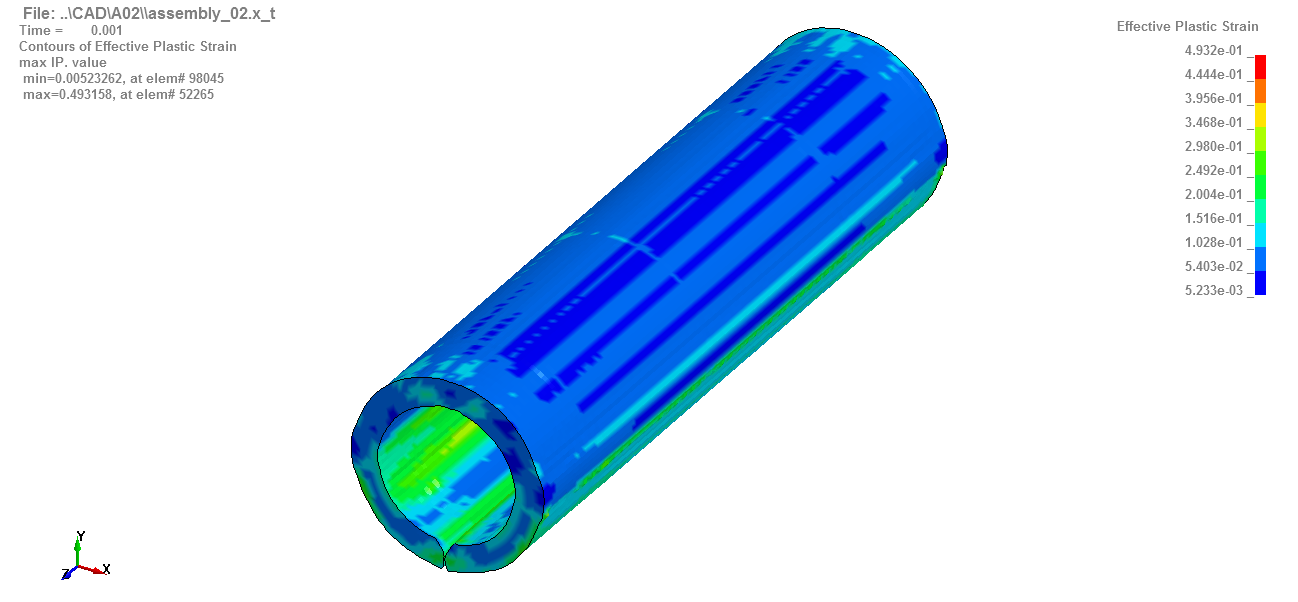
\includegraphics[width=0.75\textwidth]{src/ch4/eqv_strain_01.png}
% \captionof{figure}{Deformación plástica equivalente, primer paso}
% \label{fig:eqv_strain_01}
% \end{center}

\subsubsection{Fuerza de formado}

En las figuras \ref{fig:fuerza_formado_3d_01} y \ref{fig:fuerza_formado_3d_02} se muestran las gráficas 
correspondiente a la fuerza de formado requerida en cada una de las etapas del troquel. Se observa una 
fuerza máxima de 15,800 lbf para el primer paso, y alrededor de 94,000 lbf para el cerrado en O.\\

\begin{center}
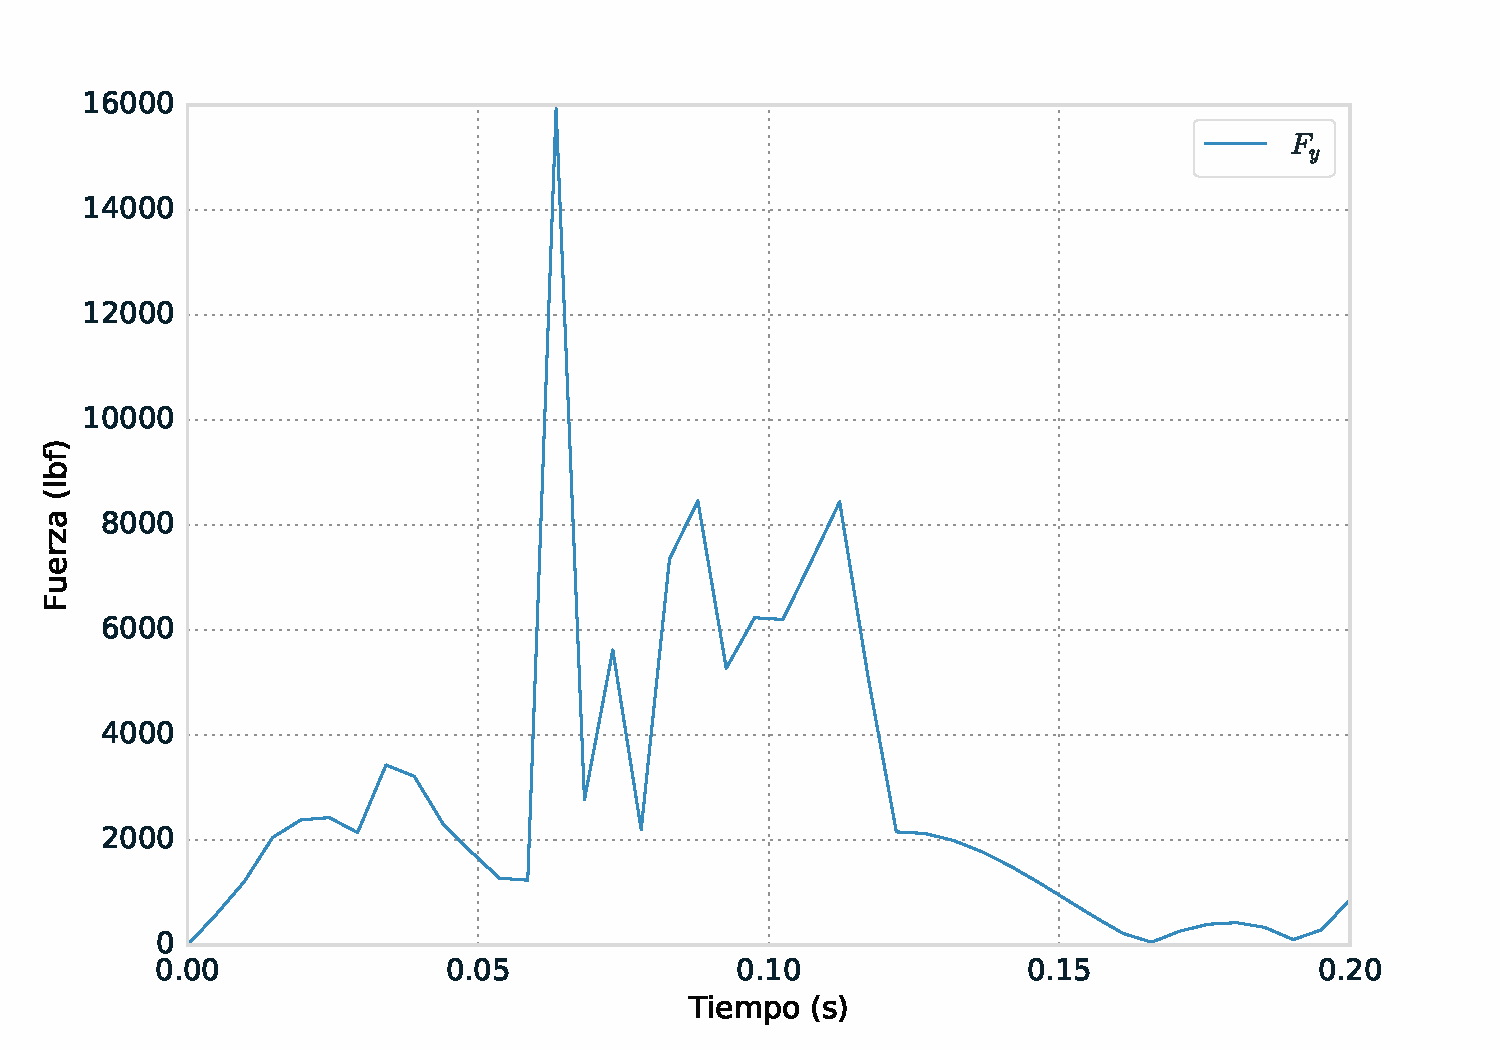
\includegraphics[width=0.75\textwidth]{src/ch4/fuerza_formado_3d_01.pdf}
\captionof{figure}{Fuerza de formado, primer paso}
\label{fig:fuerza_formado_3d_01}
\end{center}

\begin{center}
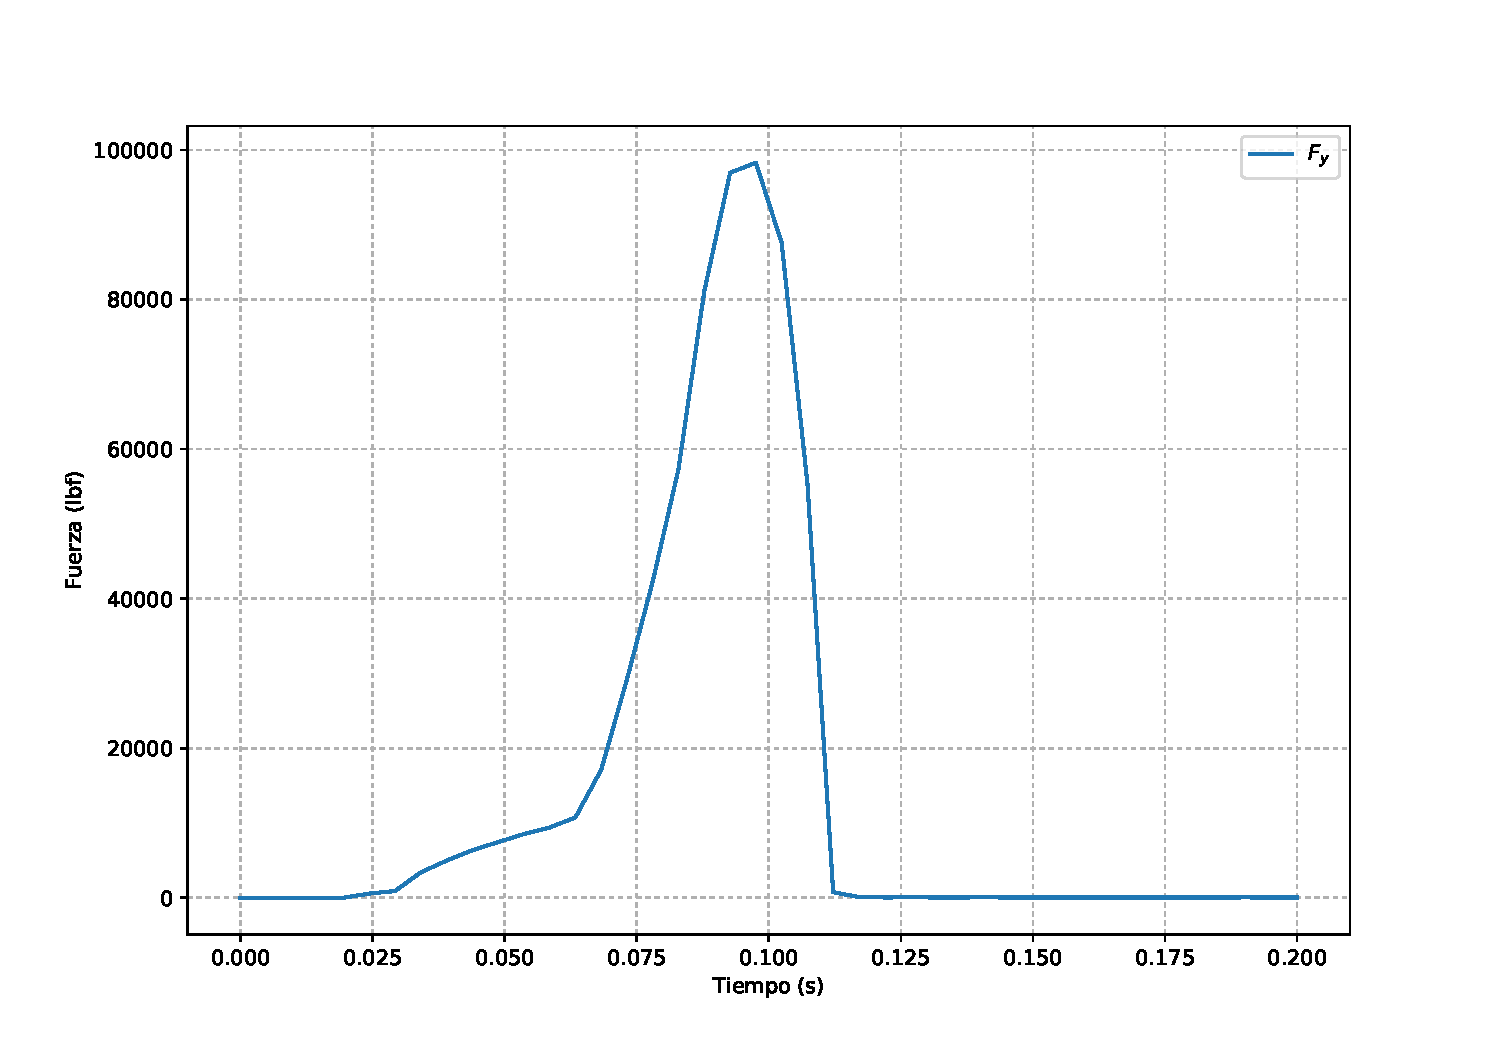
\includegraphics[width=0.75\textwidth]{src/ch4/fuerza_formado_3d_02.pdf}
\captionof{figure}{Fuerza de formado, segundo paso}
\label{fig:fuerza_formado_3d_02}
\end{center}

\subsection{Comparación 2D vs 3D}

En esta sección se presenta un análisis comparativo entre los análisis bidimensional 
y el tridimensional realizados, con el objetivo de describir particularidades respecto 
a cada enfoque y hacer énfasis en las ventajas y limitaciones de cada uno.\\

\subsubsection{Notas generales}

Es preciso hacer mención respecto a las dificultades que implica trabajar con uno u 
otro enfoque. De manera general, el modelo tridimensional representó mayores dificultades 
a la hora de ejecutar el análisis, sobre todo para cuestiones relaciones con deformaciones 
excesivas derivadas de errores de contacto entre la parte aguda de las levas formadores 
y la pieza de trabajo.\\

En el análisis bidimensional, al utilizarse un elemento (\texttt{PLANE162}) con un sólo punto 
de integración se tuvieron algunos problemas con la deformación de Hourglass, la cual implica 
un aumento excesivo en los esfuerzos resultantes y por tanto un análisis no válido, por 
lo cual se tuvieron que ajustar constantemente los parámetros de control de Hourglass.\\

En la sección \ref{sec:contactos} se describió que para definir los contactos en el 
análisis bidimensional se utiliza un contacto automático, esto implica un inconveniente 
al momento de postprocesar los resultados referentes a las fuerzas de formado, puesto 
que se tiene que hacer la lectura nodo a nodo y posteriormente sumar los resultados 
obtenidos en el historial de tiempo.\\

\subsubsection{Tiempo de cómputo}

Con tiempo de cómputo se hace referencia al tiempo transcurrido desde el inicio hasta el 
término del análisis, mismo del cual el software utilizado hace un registro. 
Es evidente que el tiempo de cómputo requerido es mayor para un modelo tridimensional, dado 
que la cantidad de ecuaciones a resolver aumenta de manera considerable.\\

Un análisis de deformación plana sin escalamiento de masa selectivo se completó en 24 minutos 
aproximadamente (0.4 horas), el mismo caso para el modelo tridimensional representó 
un costo de tiempo computacional poco mayor a 16 horas, lo cual implica una reducción de tiempo 
del 97.5\% cuando se utiliza un análisis bidimensional simplificado.

\subsubsection{Fuerza de formado}

La fuerza de formado requerida calculada para ambos casos es muy similar. Se observa también 
que la gráfica de la fuerza de formado requerida en la primera etapa para el caso tridimensional 
es bastante más oscilatoria que su equivalente bidimensional.\\

Se puede asumir que la consideración de deformación plana aproxima de manera aceptable 
los resultados obtenidos mediante el modelo tridimensional completo.

\section{Análisis de resultados experimentales }

En la sección \ref{sec:analisis-experimental} se describió el proceso de análisis experimental 
realizado con el auxilio de un prototipo. Los resultados obtenidos de las cuatro probetas 
ensayadas se pueden observar en la gráfica de la figura \ref{fig:experimental_probetas}, en 
la cual se muestra la relación carga-deformación unitaria. 
En general, las lecturas máximas que se pudieron obtener son del orden de 25 milideformaciones 
para una carga de 1600 kg. Claro está que esto representa sólo una porción del formado del primer 
paso (doblado U), pero nos sirve para comparar con los resultados arrojados por la simulación.\\

La relación carga-deformación obtenida mediante el análisis por elementos finitos se estableció 
exportando los datos de tiempo-fuerza y tiempo-deformación, para posteriormente unir estos datos 
y graficarlos acorde a la relación tiempo-fuerza-desplazamiento, para evitar \textit{desfases} en 
los datos generados, tomando además solamente los datos dentro del rango de comparación. 
Los datos de la simulación se tomaron de un análisis bidimensional, con el modelo constitutivo 
de curva multilineal y sin escalamiento de masa.\\

En la figura \ref{fig:experimental_vs_simulacion} se muestran las curvas de carga-deformación 
correspondientes a la simulación por elementos finitos y la curva experimental obtenida del 
promedio de las cuatro probetas ensayadas. En general, se observa una tendencia/comportamiento 
similar en ambos casos, con un error relativo máximo de 9\% en la sección donde la diferencia 
entre ambas curvas es notoria. Se calculó el coeficiente de correlación de Pearson para ambos conjuntos de datos, 
homogeneizando primero mediante interpolación la cantidad de datos disponibles, resultando 
un coeficiente de correlación 98\%.

\begin{center}
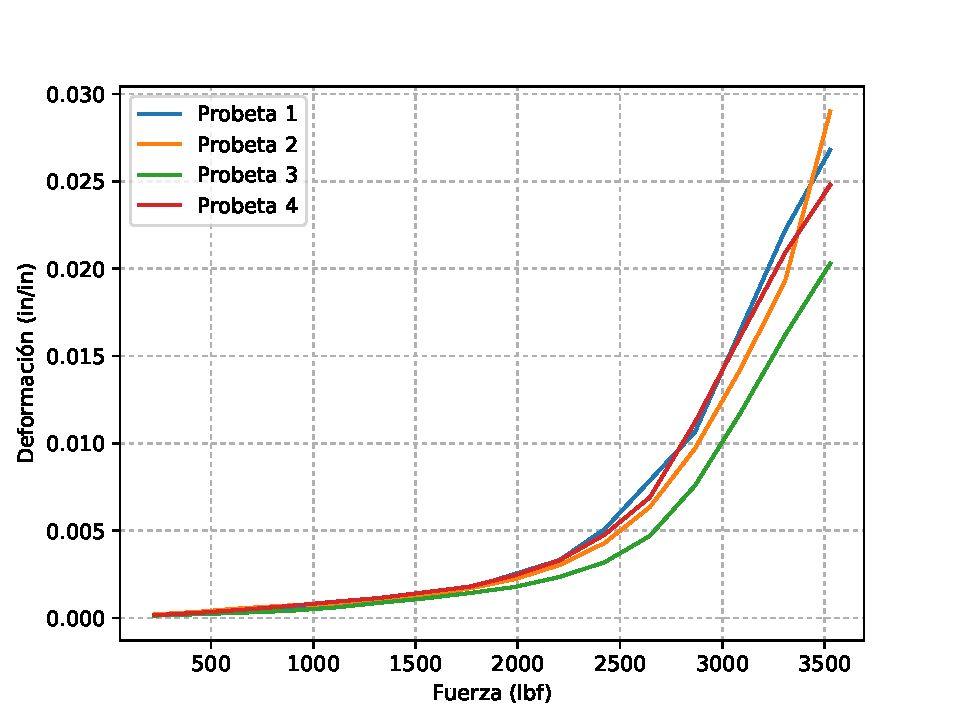
\includegraphics[width=0.85\textwidth]{src/ch4/experimental_probetas.pdf}
\captionof{figure}{Resultados experimentales de las probetas ensayadas}
\label{fig:experimental_probetas}
\end{center}

\begin{center}
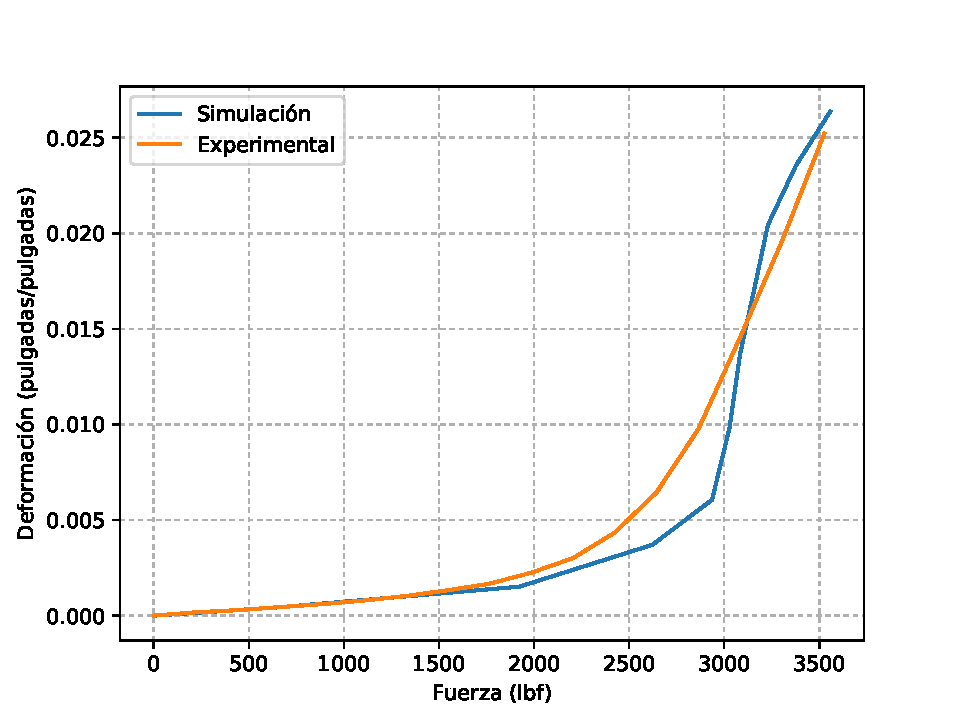
\includegraphics[width=0.85\textwidth]{src/ch4/experimental_vs_simulacion.pdf}
\captionof{figure}{Resultados experimentales vs simulación}
\label{fig:experimental_vs_simulacion}
\end{center}